\chapter{Implementacja i interpretacja wyników badań}

Do napisania pracy skorzystałem z języka skryptowego Python. Wynikało to z faktu że większość prac naukowych i badawczych jakie pisane są w obrębie dziedziny uczenia maszynowego jest tworzona właśnie w nim. Dodatkowo, skorzystałem z szeregu otwarto-źródłowych rozwiązań, takich jak:
\begin{itemize}
	\item \textit{Keras}\cite{keras} - wysokopoziomowa biblioteka do trenowania splotowych sieci neuronowych,
	\item \textit{Sikit-Learn} \cite{scikit} - biblioteka zawierająca zbiór algorytmów i narzędzi do walidacji wyników klasyfikacji,
	\item \textit{NumPy}  \cite{numpy} - biblioteka służąca do wykonania obliczeń z zakresu analizy numerycznej i algebry liniowej,
	\item \textit{Pandas}  \cite{pandas} - biblioteka służąca do manipulacji danych,
	\item \textit{Matplotlib}  \cite{matplotlib} - biblioteka służąca do wizualizacji danych,
	\item \textit{Jupyter notebook}  \cite{jupyter} - środowisko do pracy, posiadające szereg ułatwień i możliwość kolejkowania zadań.
\end{itemize}

\section{Protokół badawczy}

W niniejszej pracy przyjąłem następujący protokół badawczy - przedstawiony na rysunku \ref{fig:model_eks}. Wyróżnić można 3 główne etapy: przygotowanie danych(wczytanie danych, ich obróbka i definicja samego modelu), uczenie(podział danych i trenowanie modelu) oraz interpretacja i prezentacja wyniku.

\begin{figure}[h!]
	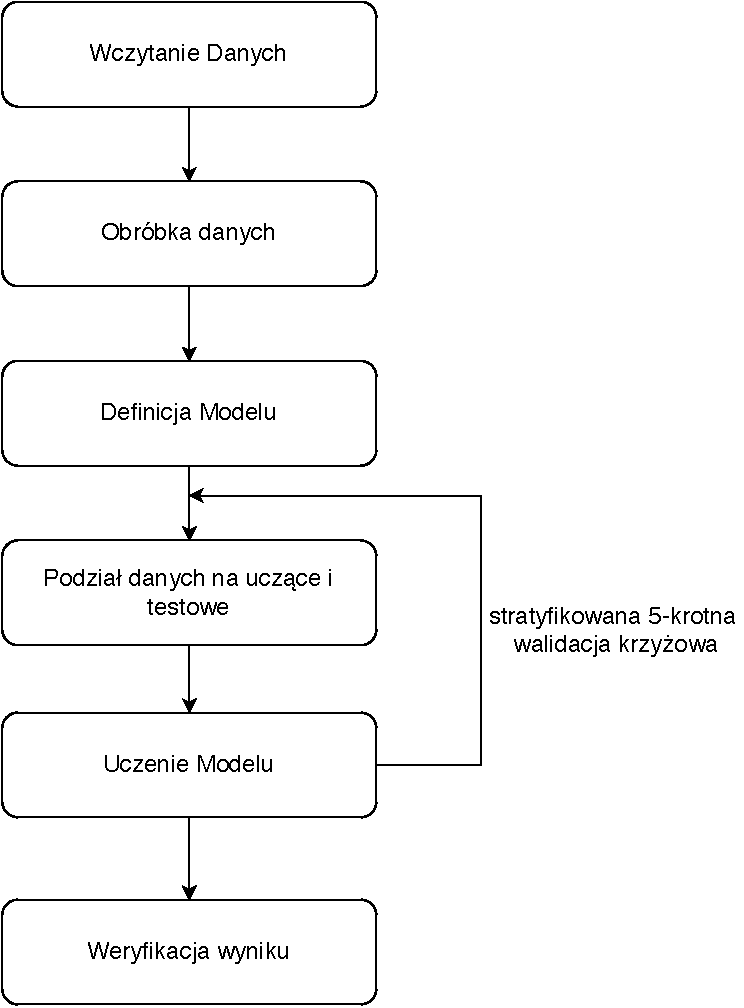
\includegraphics[width=6.5cm]{model_eksperymentu.pdf}
	\centering
	\caption{Protokół badawczy zastosowany w wykonanych eksperymentach}
	\label{fig:model_eks}
\end{figure}

\section{Implementacja środowiska  wykorzystującego maszynę wektorów nośnych}

W  pierwszej kolejności zdecydowałem się na wykorzystanie maszyny wektorów nośnych jako bazowego klasyfikatora. Idea ta jest spowodowana chęcią sprawdzenia jak klasyczne metody uczenia maszynowego sprawdzają się w porównaniu do podejścia splotowego, głębokiego.

\subsection{Przygotowanie danych}

\begin{lstlisting}[caption={Kod stworzenia ramki danych \textbf{df}}, label={lst:df}]
for filename in A_folder_list:
	categories.append(0)
	filenames.append(dir_path + '/' + A_folder + '/' + filename)
for filename in B_folder_list:
	categories.append(1)
	filenames.append(dir_path + '/' + B_folder + '/' + filename)

df = pd.DataFrame({
	'filename': filenames,
	'category': categories
})
\end{lstlisting}


Dane, a raczej pojedyncze zdjęcia zostają wczytane do Dataframe'u \textbf{df} \ref{lst:df}, skąd to potem poddawane są procesowi ekstrakcji cech. Na sam proces składa 5 osobnych funkcji, z której każda z nich przetwarza oryginalne zdjęcie. Są to kolejno:\\

\textbf{Momenty Hu} \\

Jest to  średnia ważona momentów zdjęcia opisana jako intensyfikacja pikselów w danym rejonie \cite{hu}. Pozwala to na zdefiniowanie translacji, skali i rotacji zdjęcia w odniesieniu do reszty. Opisane są wzorem \ref{eqn:hu}, a sam kod widoczny jest na listingu \ref{lst:hu}

\begin{equation}
	\begin{split}
		Hu_{1} &= \eta_{20} + \eta_{02} \\
		Hu_{2} &= (\eta_{20} - \eta_{02})^2 + 4\eta^2_{11} \\
		Hu_{3} &= (\eta_{30} - 3\eta_{12})^2 + (3\eta_{21} - \eta_{02})^2 \\
		Hu_{4} &= (\eta_{30} + \eta_{12})^2 + (\eta_{21} + \eta_{02})^2 \\
		Hu_{5} &= (\eta_{30} - 3\eta_{12})(\eta_{30} - \eta_{12})\left [ (\eta_{30} + \eta_{12})^2 - 3(\eta_{21} + \eta_{03})^2 \right ] +\\
		 &+ (3\eta_{21} - \eta_{03})(\eta_{21}+\eta_{03})\left [3(\eta_{30} + \eta_{12})^2-(\eta_{21} + \eta_{03})^2 \right ] \\
		 Hu_{6} &= (\eta_{20}-\eta_{02})\left [ (\eta_{30} + \eta_{12})^2 - (\eta_{21} + \eta_{03})^2\right ] +4\eta_{11}(\eta_{30}+\eta_{12})(\eta_{21} + \eta_{03}) \\
		 Hu_{7} &= (3\eta_{21} - \eta_{03})(\eta_{30}+\eta_{12})\left [(\eta_{30}+\eta_{12})^2-3(\eta_{21}+\eta_{03})^2 \right ] -\\
		  &- (\eta_{30}-3\eta_{12})(\eta_{21} + \eta_{03}) \left [3(\eta_{30}+\eta_{12})^2-(\eta_{21} + \eta_{03})^2 \right ]
	\end{split}
	\label{eqn:hu}
\end{equation}

\begin{lstlisting}[caption={Implementacja ekstrakcji momentów hu}, label={lst:hu}]
def ft_hu_moments(image):
	image = cv2.cvtColor(image, cv2.COLOR_BGR2GRAY)
	hu_moments = cv2.HuMoments(cv2.moments(image)).flatten()
	hu_moments = scaler.fit_transform(hu_moments.reshape(-1, 1))
	hu_moments = hu_moments.flatten()
	return hu_moments
\end{lstlisting}

\textbf{Cechy Haralicka} \\

Zaproponowany przez Roberta Haralicka  w 1979 roku \cite{harlick} zestaw cech bazuje na czarno-białej reprezentacji oryginalnego zdjęcia. Na jej podstawie generuje się tablicę współwystąpień, określaną skrótem \textbf{GLCM}, z której to w dalszej kolejności wylicza się zestaw 13 cech opisanych następującymi wzorami \ref{eqn:haralicka}, których implementacja widoczna jest w listingu \ref{lst:haralick}. Ich zadaniem jest określenie \textit{tekstury} zdjęcia.

\begin{equation}
	\begin{aligned}[c]
		\begin{split}
			f_{1} &=\sum_{i=0}^{G-1}\sum_{j=0}^{G-1} P(i,j)^2 \\
			f_{2} &=\sum_{i=0}^{G-1}\sum_{j=0}^{G-1} P(i,j)*(i-j)^2 \\
			f_{3} &=\sum_{i=0}^{G-1}\sum_{j=0}^{G-1} P(i,j)\left [ \frac{(i-\mu_{i})(j-\mu_{j})}{\sqrt{(\delta^2_{i})(\delta^2_{j})}} \right ]\\
			f_{4} &=\sum_{i=0}^{G-1}\sum_{j=0}^{G-1} P(i,j)*\left | i-j \right | \\
			f_{5} & =\sum_{i=0}^{G-1}\sum_{j=0}^{G-1} \frac{P(i,j)}{1+(i+j)^2}\\
			f_{6} &=\sum_{i=0}^{G-1}\sum_{j=0}^{G-1} P(i,j)*(i-\mu)^2
			\end{split}
		\end{aligned}
		\begin{aligned}[c]
			\begin{split}
				f_{7} &=-\sum_{i=0}^{G-1}\sum_{j=0}^{G-1} P(i,j)\log(P(i,j))\\
				f_{8} &=\sqrt{\sum_{i=0}^{G-1}\sum_{j=0}^{G-1} P(i,j)^2 }\\
				f_{9} &=\sum_{i=2}^{2N_{g}}ip_{x+y}(i)\\
				f_{10} &=-\sum_{i=2}^{2N_{g}}p_{x+y}(i)\log(p_{x+y}(i))\\
				f_{11} &=\sum_{i=2}^{2N_{g}}(i - f_{10})^2 p_{x+y}(i)\\
				f_{12} &=Var\left [ p_{x-y} \right ]\\
				f_{13} &=-\sum_{i=0}^{N_{g}-1}p_{x-y}(i)\log(p_{x-y}(i))
			\end{split}
		\end{aligned}
	\label{eqn:haralicka}
\end{equation}

\begin{lstlisting}[caption={Implementacja przeliczania cechy Haralicka}, label={lst:haralick}]
def ft_haralick(image):
	image = cv2.cvtColor(image, cv2.COLOR_BGR2GRAY)
	haralick = mahotas.features.haralick(image).mean(axis=0)
	haralick = scaler.fit_transform(haralick.reshape(-1, 1))
	haralick = haralick.flatten()
	return haralick
\end{lstlisting}

\textbf{Histogram kolorów} \\

Kolejną z rozpatrywanych cech jest histogram kolorów zdjęcia. Sam histogram to po prostu graficzny sposób przedstawiania rozkładu empirycznego cechy - dla zdjęcia będą to oczywiście rozkłady każdego z podstawowych kolorów(R - dla czerwonego, G - dla zielonego i B - dla niebieskiego). Całość została graficznie pokazana na rysunku \ref{fig:lena}, oraz zaimplementowana w listingu \ref{lst:hist}.

\begin{figure}[h!]
	\centering
	\subfloat{{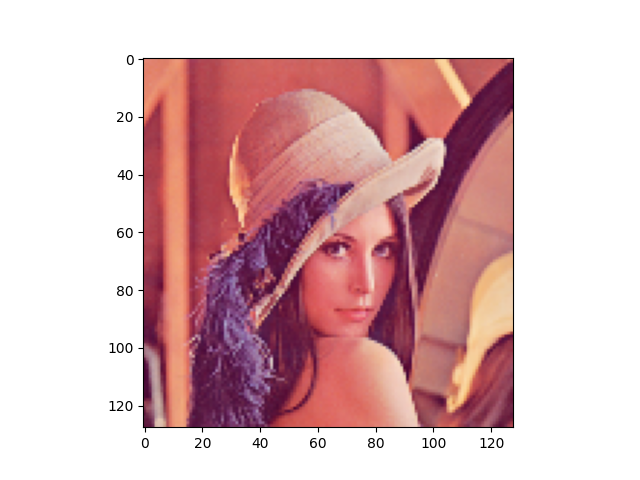
\includegraphics[width=7cm]{org.png} }}
	\qquad
	\subfloat{{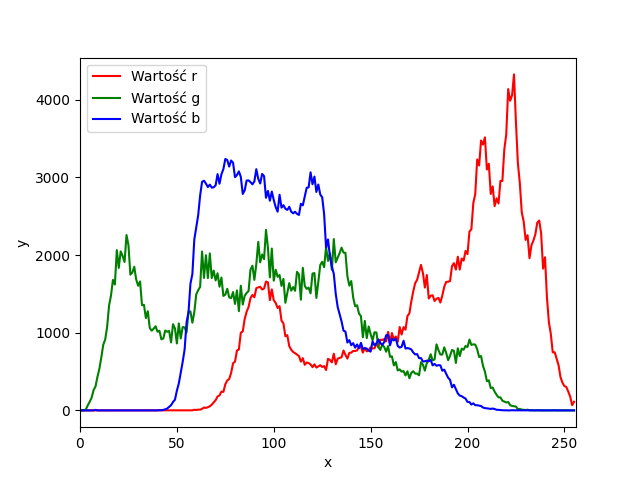
\includegraphics[width=7cm]{histogram.png} }}
	\caption{Zdjęcie i odpowiadający mu histogram kolorów}
	\label{fig:lena}
\end{figure}

\begin{lstlisting}[caption={implementacja wyliczania histogramu kolorów}, label={lst:hist}]
def ft_histogram(image, mask=None):
	image = cv2.cvtColor(image, cv2.COLOR_BGR2HSV)
	hist  = cv2.calcHist([image], [0, 1, 2], None, [8, 8, 8], [0, 256, 0, 256, 0, 256])
	cv2.normalize(hist, hist)
	return hist.flatten()
\end{lstlisting}

\textbf{Histogram gradientów} \\
 
Technika ta opracowana w 2005 roku \cite{hog} służy w większości do rozpoznawania sylwetek głównych obiektów na zdjęciach. Polega ona na przeglądaniu kwadratów o wielkości $8 \times 8$ pikseli i staraniu się w nich o detekcje krawędzi, poprzez badanie wielkości różnic pomiędzy kolorami sąsiednich pikseli. Całość została graficznie przedstawiona na obrazku \ref{fig:hog}, a kod samej funkcji realizującej to zadanie jest widoczny w listing \ref{lst:hog}.

\begin{figure}[h!]
	\centering
	\subfloat{{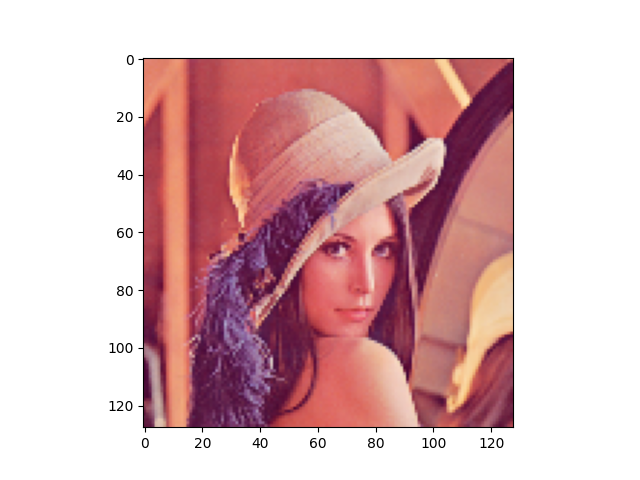
\includegraphics[width=7cm]{org.png} }}
	\qquad
	\subfloat{{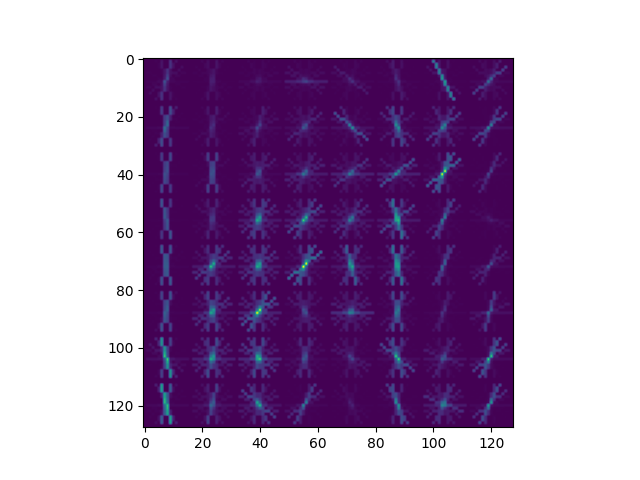
\includegraphics[width=7cm]{hog.png} }}
	\caption{Zdjęcie oryginalne i po wykonaniu na nim histogramu gradientów}
	\label{fig:hog}
\end{figure}

\begin{lstlisting}[caption={Implementacja wyliczania histogramu gradientów}, label={lst:hog}]
def ft_hog(image):
	image = cv2.cvtColor(image, cv2.COLOR_BGR2GRAY)
	hog_features, hog_image = hog(image, block_norm='L2-Hys', 
															  pixels_per_cell=(16, 16), cells_per_block=(1, 1), 
															  visualize=True)
	return hog_features, hog_image
\end{lstlisting}

\textbf{Analiza poziomu błędu} \\

Jest to funkcjonalność którą opisywałem już w rozdziale 3. Podsumowując korzystanie z algorytmu ELA(z ang. \textit{Error Level Analysis}), opisanego w pracy N. Krawetza z 2007 roku\cite{hacker} polega na wykorzystaniu właściwości zapisywania formatu *.JPEG w różnych jakościach. Ideą algorytmu ELA, w wersji którą zaimplementowałem i wykorzystałem, jest zapisanie zdjęcia podwójnie z kompresją pomiędzy $\sim85\%$ - $\sim95\%$, a następnie \textit{dodanie} różnic. Całość widoczna jest graficznie na rysunku \ref{fig:ela}, a kod został przedstawiony na listingu \ref{lst:ela}.

\begin{figure}[h!]
	\centering
	\subfloat{{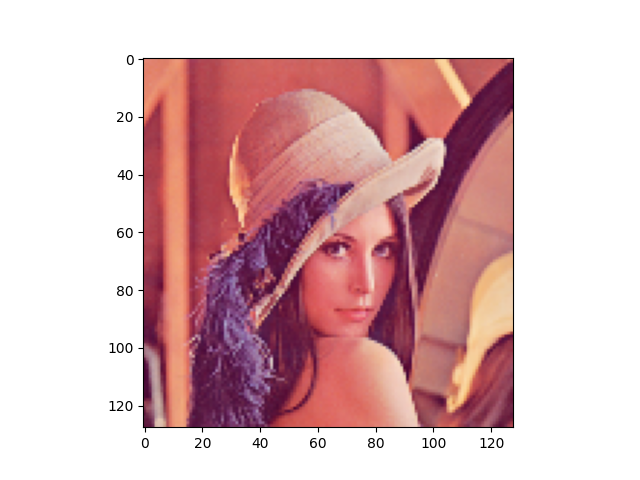
\includegraphics[width=7cm]{org.png} }}
	\qquad
	\subfloat{{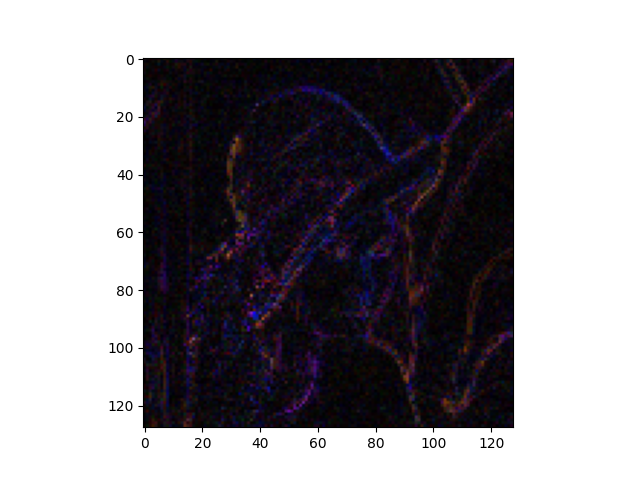
\includegraphics[width=7cm]{ela.png} }}
	\caption{Zdjęcie oryginalne i po zastosowaniu na nim algorytmu ELA}
	\label{fig:ela}
\end{figure}

\begin{lstlisting}[caption={Implementacja realizacji analizy poziomu błędów}, label={lst:ela}]
def ft_ela(image):
	image = cv2.cvtColor(image, cv2.COLOR_BGR2RGB)
	ans = []
	for i in range(86, 96):
		im = Image.fromarray(image)
		im.save(f'tmp_{i}.jpg', 'JPEG', quality=i)
		resaved_im = Image.open(f'tmp_{i}.jpg')
		
		ela_im = ImageChops.difference(im, resaved_im)
		
		extrema = ela_im.getextrema()
		max_diff = max([ex[1] for ex in extrema])
		if max_diff == 0:
		max_diff = 1
		scale = 255.0 / max_diff
		ans.append(max_diff)
	
	ela_im = ImageEnhance.Brightness(ela_im).enhance(scale)
	ret = numpy.array([ans]).flatten() / 255
	
	return ret, ela_im
\end{lstlisting}

Podsumowując, pojedyncze zdjęcie po ekstrakcji cech przez opisane powyżej funkcję jest definiowane przez zestaw $1118$ liczb. Udział poszczególnych cech widoczny jest w tabeli \ref{tab:pdst}.  Warto tutaj też dodać również, że opisane cechy są znormalizowane, to jest ich zakres wynosi $\left [ 0,1 \right ]$. Funkcję takie jak histogram kolorów, histogram gradientów i ELA normalizowane są niejako automatycznie(znany jest zakres możliwych do przyjęcia wartości), ale dla funkcji momentów hu i cech haralicka z racji, że nie maja one zakresu rzuconych wyników, zastosowany został \textit{MinMaxScaler}. Jego zasada jest dość prosta - znajduję w zadanym zakresie minimalną i maksymalną wartość, a następnie mapuje resztę wartości w odniesieniu do nich.  \\

\begin{table}[h!]
	\centering
	\begin{tabular}{l|l|l|}
		\cline{2-3}
		& Ilość elementów & Procentowy udział w całości \\ \hline
		\multicolumn{1}{|l|}{\textbf{Wielkość całego wektora}} & \textbf{1118} & \textbf{100\%} \\ \hline
		\multicolumn{1}{|l|}{Momenty Hu}            & 7               & 0.63\%                      \\ \hline
		\multicolumn{1}{|l|}{Cechy Haralicka}       & 13              & 1.16\%                      \\ \hline
		\multicolumn{1}{|l|}{Histogram kolorów}     & 512             & 45.80\%                     \\ \hline
		\multicolumn{1}{|l|}{Histogram gradientów}  & 576             & 51.52\%                     \\ \hline
		\multicolumn{1}{|l|}{Analiza poziomu błędu} & 10              & 0.89\%                      \\ \hline
	\end{tabular}
	\caption{Udział poszczególnych funkcji ekstrakcji cech w konstrukcji wektora opisującego pojedyncze zdjęcie}
	\label{tab:pdst}
\end{table}

Dodatkowo z racji dużej ilości danych opisujący pojedynczą próbkę, zastosowałem dekompozycję przy pomocy analizy głównych składowych \cite{pca}, którą to dokładniej opisałem w rozdziale 2 niniejszej pracy.  Redukcja PCA odbyła z 1118 elementów do 700, co daję redukcję o $\sim37\%$.

\subsection{Definicja i uczenie modeli}

Na potrzeby maszyny wektorów nośnych przygotowane zostały 5 podstawowych wersji klasyfikatora SVM \cite{hands_on}: \textit{SVM linear}, \textit{SVM poly}, \textit{SVM rbf}, \textit{SVM sigmoid}(widoczne na listingu \ref{lst:clf}). Różnią się one tylko jądrem, a co za tym idzie - poszukiwaną funkcją na podstawie której budowana jest hiperpłaszczyzna separująca.

\begin{lstlisting}[caption={Możliwe klasyfikactory dla SVM'a}, label={lst:clf}]
clfs = {
	"SVM linear": SVC(kernel='linear', probability=True, random_state=odp, verbose=True),
	"SVM poly": SVC(kernel='poly', probability=True, random_state=odp, verbose=True),
	"SVM rbf": SVC(kernel='rbf', probability=True, random_state=odp, verbose=True),
	"SVM sigmoid": SVC(kernel='sigmoid', probability=True, random_state=odp,verbose=True)
}
\end{lstlisting}

Same uczenie jest wykonywane zgodnie z zasadami 5-krotnej stratyfikowanej walidacji krzyżowej, opisanej szczegółowo w rozdziale 2 niniejszej pracy. Oprócz tego na każdym etapie liczone sa wszelkie zdefiniowane w rozdziale 2 miary określające prace modelu. Kod opisanych sytuacji widoczny jest na listingu \ref{lst:fit}.

\begin{lstlisting}[caption={Implementacja trenowanie modelów z zastosowaniem 5-krotnej startyfikowanej walidacji krzyżowej}, label={lst:fit}]
for fold_id, (train_index, test_index) in enumerate(kf.split(features, labels)):
	for clf_idx, clf_name in enumerate(clfs):
		clf = clone(clfs[clf_name])
		clf.fit(features[train_index], labels[train_index])
		y_pred = clf.predict(features[test_index])

		accuracy, precision, recall, fscore = countStats(labels[test_index], y_pred)
		cm = confusion_matrix(labels[test_index], y_pred)
\end{lstlisting}

\subsection{Interpretacja uzyskanych wyników}

Poniżej przedstawiam wyniki uzyskane dla poszczególnych zbiorów danych jakie zostały użyte podczas pisania pracy. \\

\textbf{Zbiór danych CASIA} \\

Same wyniki są przestawione w tabeli \ref{tab:result}. Podano tam wartość danej statystyki(liczoną jako średnią z pięciu przebiegów) oraz dodatkowo odchylenie standardowe.
\begin{table}[h!]
	\centering
	\begin{tabular}{|l|l|l|l|l|}
		\hline
		\textbf{Kernel} & \textbf{Dokładność} & \textbf{Precyzja} & \textbf{Czułość} & \textbf{Miara \textit{F}} \\ \hline
		\textit{linear}  & 0.710 (0.01) & 0.664 (0.01) & 0.581 (0.01) & 0.619 (0.01) \\ \hline
		\textit{poly}    & 0.647 (0.01) & 0.618 (0.01) & 0.343 (0.01) & 0.441 (0.01) \\ \hline
		\textit{rbf}     & 0.725 (0.00) & 0.669 (0.00) & 0.638 (0.01) & 0.653 (0.00) \\ \hline
		\textit{sigmoid} & 0.662 (0.01) & 0.593 (0.01) & 0.538 (0.01) & 0.564 (0.01) \\ \hline
	\end{tabular}
	\caption{Wartości miar w zależności od przyjętego jądra modelu SVM, dla zbioru danych CASIA}
	\label{tab:result}
\end{table}

Oprócz tego dla każdej z miar zostały wykonane parowe testy statystyczne w oparciu o statystykę t-studenta \cite{stata}. Wyniki zostały przedstawione w tablicy \ref{tab:result_c}.

\begin{table}[h!]
	\centering
	\begin{tabular}{l|l|l|l|l|l|l|l|l|l|l|l|l|l|l|l|l|}
		\cline{2-17}
		&
		\multicolumn{4}{c|}{\textbf{Dokładność}} &
		\multicolumn{4}{c|}{\textbf{Precyzja}} &
		\multicolumn{4}{c|}{\textbf{Czułość}} &
		\multicolumn{4}{c|}{\textbf{Miara \textit{F}}} \\ \cline{2-17} 
		\textbf{} &
		\textbf{lin} &
		\textbf{pol} &
		\textbf{rbf} &
		\textbf{sig} &
		\textbf{lin} &
		\textbf{pol} &
		\textbf{rbf} &
		\textbf{sig} &
		\textbf{lin} &
		\textbf{pol} &
		\textbf{rbf} &
		\textbf{sig} &
		\textbf{lin} &
		\textbf{pol} &
		\textbf{rbf} &
		\textbf{sig} \\ \hline
		\multicolumn{1}{|l|}{\textbf{lin}}  & 0 & 1 & 0 & 1 & 0 & 1 & 0 & 1 & 0 & 1 & 0 & 1 & 0 & 1 & 0 & 1 \\ \hline
		\multicolumn{1}{|l|}{\textbf{pol}}    & 0 & 0 & 0 & 0 & 0 & 0 & 0 & 1 & 0 & 0 & 0 & 0 & 0 & 0 & 0 & 0 \\ \hline
		\multicolumn{1}{|l|}{\textbf{rbf}}     & 1 & 1 & 0 & 1 & 0 & 1 & 0 & 1 & 1 & 1 & 0 & 1 & 1 & 1 & 0 & 1 \\ \hline
		\multicolumn{1}{|l|}{\textbf{sig}} & 0 & 1 & 0 & 0 & 0 & 0 & 0 & 0 & 0 & 1 & 0 & 0 & 0 & 1 & 0 & 0 \\ \hline
	\end{tabular}
	\caption{Wynik działania dla wszystkich miar w oparciu o parowe testy statystyczne wykonane na zbiorze danych CASIA }
	\label{tab:result_c}
\end{table}

Po analizie wyników można stwierdzić że najlepszy rezultat dla zbioru danych CASIA osiągnął kernel \textbf{RBF}:
\begin{itemize}
	\item Dokładność: \textbf{0.725 (0.00)},
	\item Precyzja: \textbf{0.669 (0.00)},
	\item Czułość: \textbf{0.638 (0.01)},
	\item Miara \textit{F}: \textbf{0.653 (0.00)}. \\
\end{itemize}
Tablica błędów prezentuję się następująco(rysunek \ref{fig:rbf_cm_casia}):

\begin{figure}[h!]
	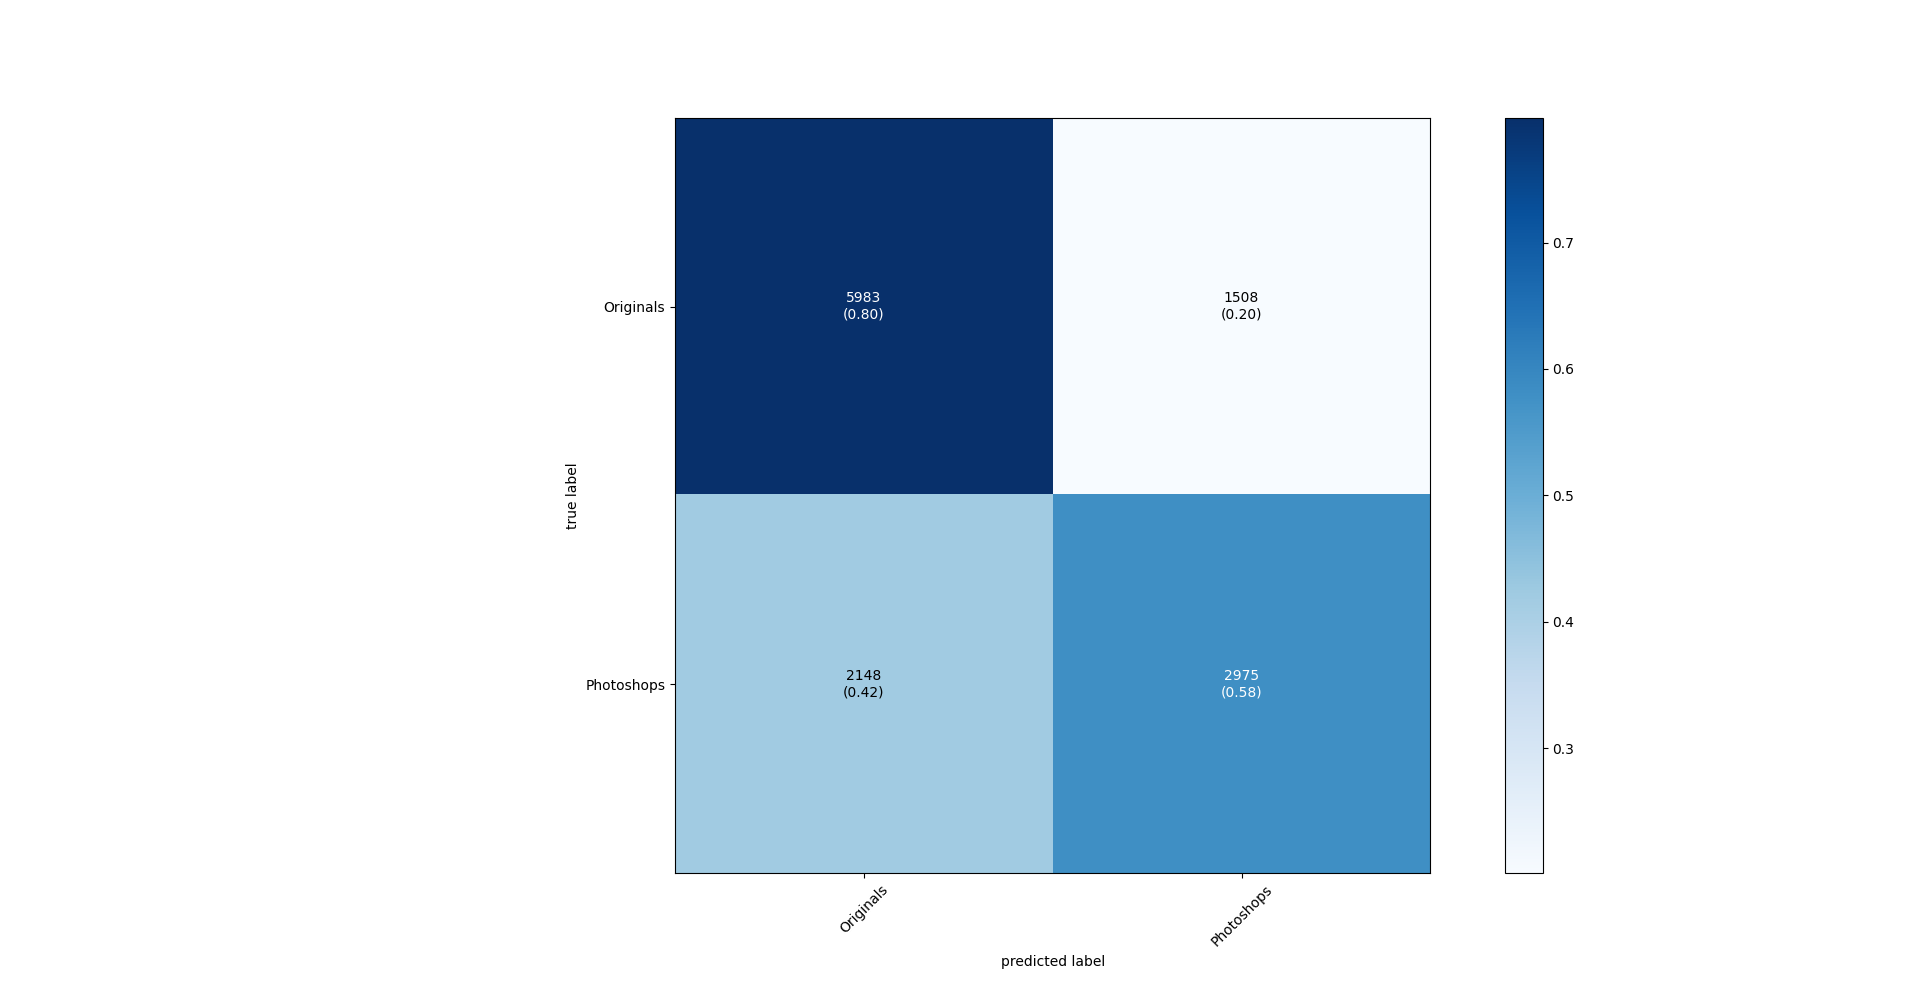
\includegraphics[width=10cm]{SVM_CASIA_CM.png}
	\centering
	\caption{Tablica błędów dla SVM'a z jądrem RBF, trenowanego na zbiorze danych CASIA}
	\label{fig:rbf_cm_casia}
\end{figure}

\textbf{Zbiór danych PS-Battles} \\

Same wyniki są przedstawione w tabeli \ref{tab:result_p}. Podano tam wartość danej statystyki(liczoną jako średnią z pięciu przebiegów) oraz dodatkowo odchylenie standardowe.
\begin{table}[h!]
	\centering
	\begin{tabular}{|l|l|l|l|l|}
		\hline
		\textbf{Kernel} & \textbf{Dokładność} & \textbf{Precyzja} & \textbf{Czułość} & \textbf{Miara \textit{F}} \\ \hline
		\textit{linear}  & 0.580 (0.01) & 0.590 (0.01) & 0.527 (0.01) & 0.557 (0.01) \\ \hline
		\textit{poly}    & 0.482 (0.01) & 0.468 (0.01) & 0.264 (0.01) & 0.337 (0.01) \\ \hline
		\textit{rbf}     & 0.529 (0.01) & 0.530 (0.01) & 0.504 (0.01) & 0.517 (0.01) \\ \hline
		\textit{sigmoid} & 0.541 (0.00) & 0.543 (0.00) & 0.527 (0.01) & 0.535 (0.01) \\ \hline
	\end{tabular}
	\caption{Wartości miar w zależności od przyjętego jądra modelu SVM, dla zbioru danych PS-Battles}
	\label{tab:result_p}
\end{table}

Oprócz tego dla każdej z miar zostały wykonane parowe testy statystyczne w oparciu o statystykę t-studenta \cite{stata}. Wyniki zostały przedstawione w tablicy \ref{tab:result_pp}

\begin{table}[h!]
	\centering
	\begin{tabular}{l|l|l|l|l|l|l|l|l|l|l|l|l|l|l|l|l|}
		\cline{2-17}
		&
		\multicolumn{4}{c|}{\textbf{Dokładność}} &
		\multicolumn{4}{c|}{\textbf{Precyzja}} &
		\multicolumn{4}{c|}{\textbf{Czułość}} &
		\multicolumn{4}{c|}{\textbf{Miara \textit{F}}} \\ \cline{2-17} 
		\textbf{} &
		\textbf{lin} &
		\textbf{pol} &
		\textbf{rbf} &
		\textbf{sig} &
		\textbf{lin} &
		\textbf{pol} &
		\textbf{rbf} &
		\textbf{sig} &
		\textbf{lin} &
		\textbf{pol} &
		\textbf{rbf} &
		\textbf{sig} &
		\textbf{lin} &
		\textbf{pol} &
		\textbf{rbf} &
		\textbf{sig} \\ \hline
		\multicolumn{1}{|l|}{\textbf{lin}}  & 0 & 1 & 1 & 1 & 0 & 1 & 1 & 1 & 0 & 1 & 1 & 0 & 0 & 1 & 1 & 1 \\ \hline
		\multicolumn{1}{|l|}{\textbf{pol}}    & 0 & 0 & 0 & 0 & 0 & 0 & 0 & 0 & 0 & 0 & 0 & 0 & 0 & 0 & 0 & 0 \\ \hline
		\multicolumn{1}{|l|}{\textbf{rbf}}     & 0 & 1 & 0 & 0 & 0 & 1 & 0 & 0 & 0 & 1 & 0 & 0 & 0 & 1 & 0 & 0 \\ \hline
		\multicolumn{1}{|l|}{\textbf{sig}} & 0 & 1 & 1 & 0 & 0 & 1 & 1 & 0 & 0 & 1 & 1 & 0 & 0 & 1 & 1 & 0 \\ \hline
	\end{tabular}
	\caption{Wynik działania dla wszystkich miar w oparciu o parowe testy statystyczne wykonane na zbiorze danych PS-Battles }
	\label{tab:result_pp}
\end{table}

Po analizie wyników można stwierdzić że najlepszy rezultat dla zbioru danych PS-Battles osiągnął kernel \textbf{linear}:
\begin{itemize}
	\item Dokładność: \textbf{0.580 (0.00)},
	\item Precyzja: \textbf{0.590 (0.00)},
	\item Czułość: \textbf{0.527 (0.01)},
	\item Miara \textit{F}: \textbf{0.557 (0.00)}. \\
\end{itemize}
Tablica błędów prezentuję się następująco(rysunek \ref{fig:linear_cm_casia}):

\begin{figure}[h!]
	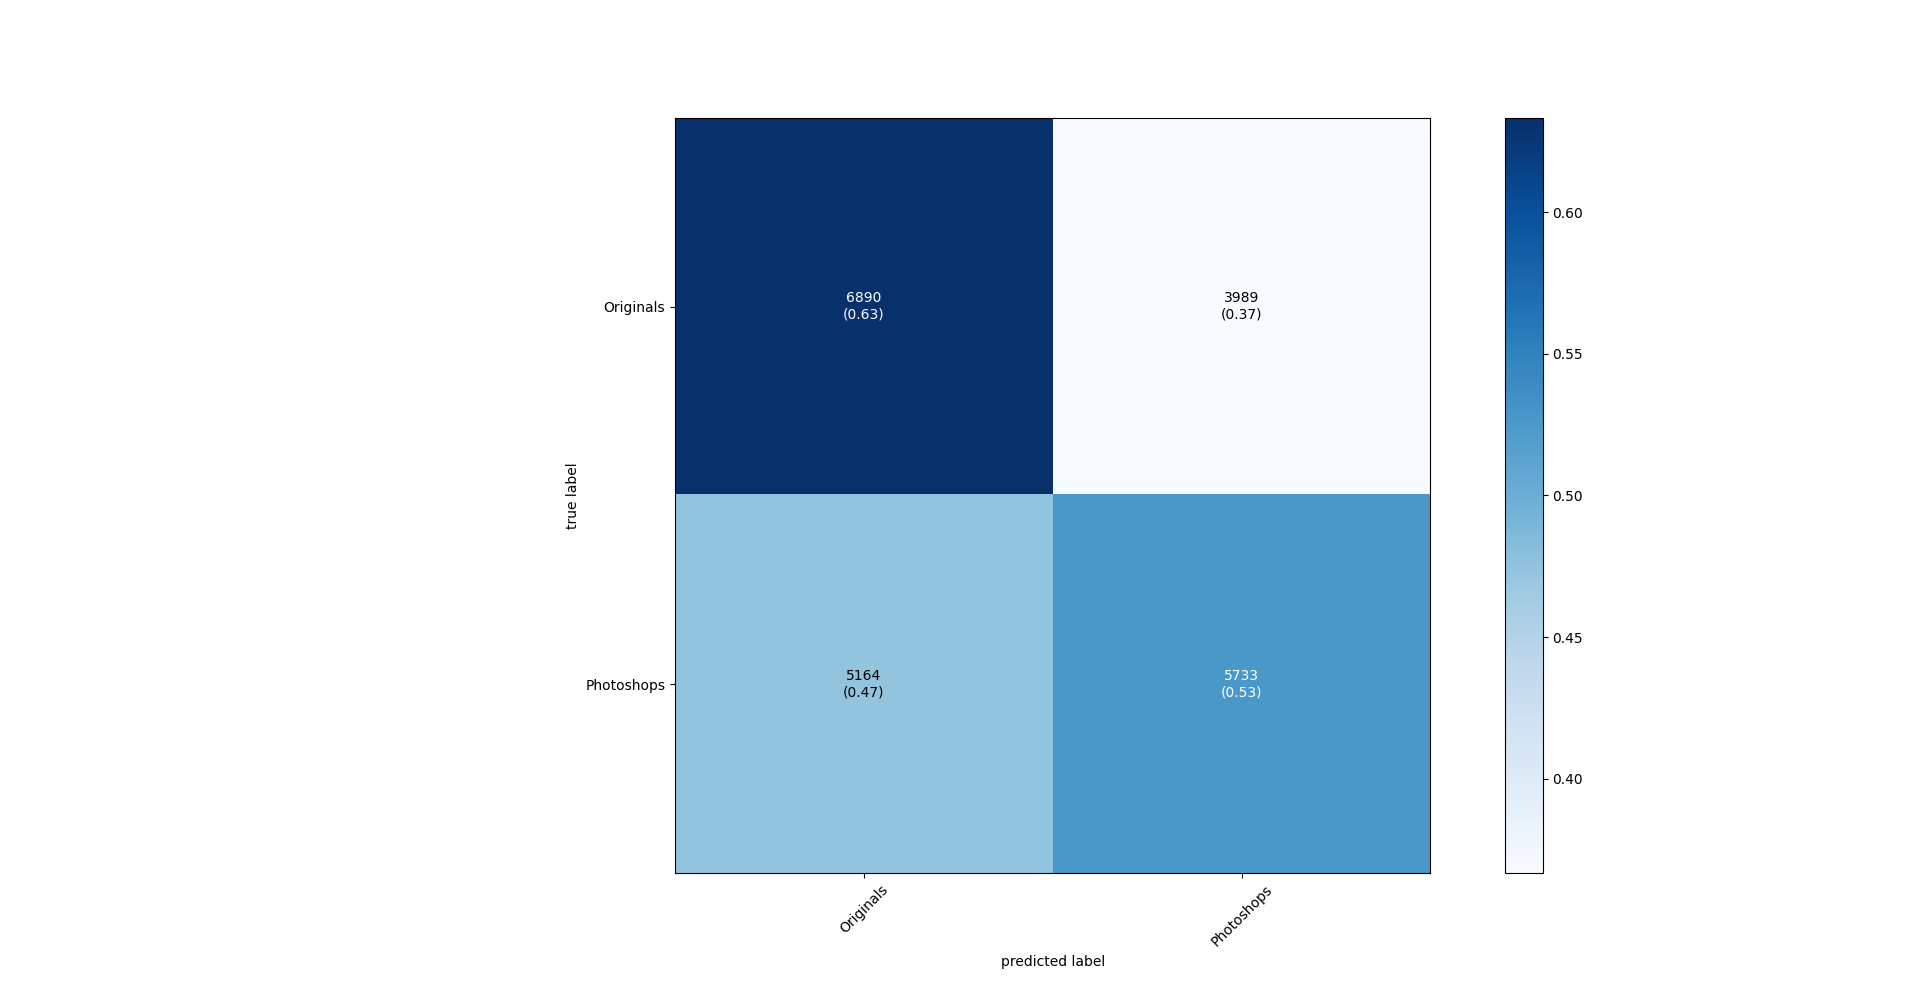
\includegraphics[width=10cm]{SVM_PHOTO_CM.png}
	\centering
	\caption{Tablica błędów dla SVM'a z jądrem \textit{Linear}, trenowanego na zbiorze danych PS-Battles}
	\label{fig:linear_cm_casia}
\end{figure}

\section{Implementacja środowiska wykorzystującego istniejące architektury sieci}

Do następnej części postanowiłem skorzystać z klasycznego modelu ucznia głębokiego, jakim jest VGG Net, wykorzystując w tym momencie technikę transferu wiedzy opisaną w rozdziale 2 . W skrócie, polega ona na wykorzystaniu modelu o już nauczonych wagach, które to częściowo są zamrażane, przez co nie zmieniają się w procesie uczenia. Schemat modelu dostępny jest na rysunku \ref{fig:vgg16}.

\begin{figure}[h!]
	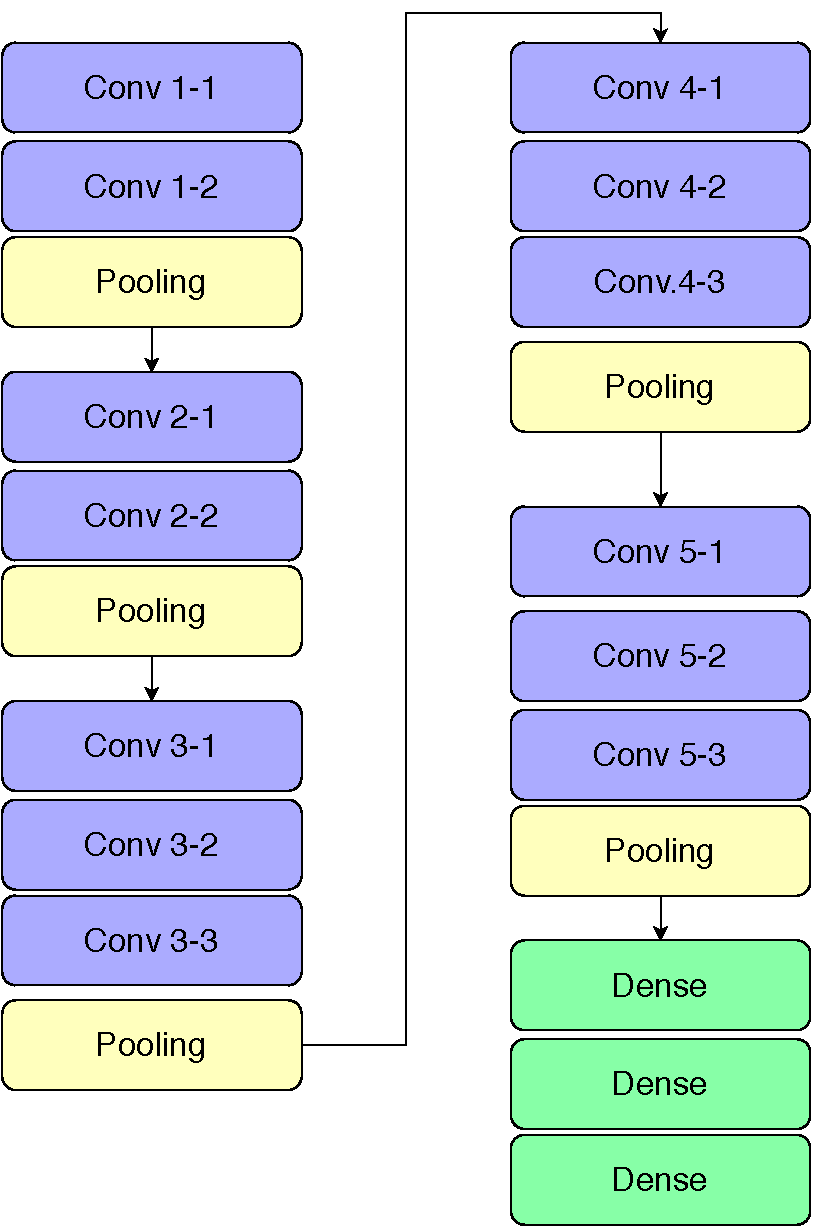
\includegraphics[width=10cm]{vgg16.pdf}
	\centering
	\caption{Schemat modelu VGG16}
	\label{fig:vgg16}
\end{figure}

\subsection{Przygotowanie danych}

Dane w początkowej fazie swojej żywotności traktowane są dokładnie tak samo jak przy maszynie wektorów nośnych(zgodnie z listingiem \ref{lst:df}). Tym razem jednak zamiast w dalszej części skupić się na kolejnych pięciu funkcjach odpowiedzialnych za ekstrakcje cech, na wejście sieci zawierającej VGG Net trafia wynik operacji algorytmu ELA na całym zbiorze. Kod tego rozwiązania dostępny jest na listingu \ref{lst:ela} oraz w formie graficznej na rysunku \ref{fig:ela}. Warto tutaj zaznaczyć że wielkość zdjęcia została przyjęta na $150 \times 150$.

\subsection{Definicja i uczenie modelu}

Wykorzystałem 16-warstwowy model VGG Netu - powodem było duża ilość parametrów, które wraz z kolejnymi wersjami(dodającymi kolejne warstwy), nie gwarantują dużo lepszych wyników \cite{vgg}. Na jego podstawie zbudowałem model odpowiadający mojej ilości klas, który to składał się z warstwy VGG Netu, pojedynczej warstwy Dropout i dwóch warstw w pełni połączonych. Graficzną reprezentację tego schematu można zobaczyć na rysunku \ref{fig:my_vgg16}.

\begin{figure}[h!]
	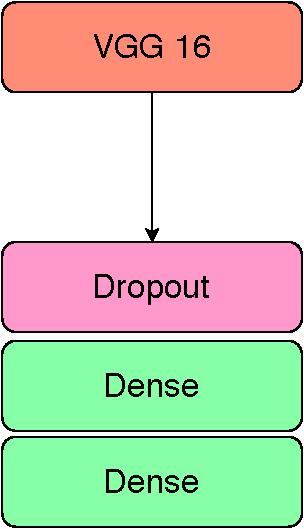
\includegraphics[width=3cm]{my_vgg16.pdf}
	\centering
	\caption{Schemat modelu zbudowanego o VGG16}
	\label{fig:my_vgg16}
\end{figure}

Same uczenie opiera o szereg parametrów, takich jak: spodziewana ilość epok, funkcja aktywacji, czy funkcja optymalizująca wykorzystująca propagację wsteczną. Ich wartości zostały przedstawione na listingu \ref{lst:param}.

\begin{lstlisting}[caption={Parametry pracy modelu opartego o transfer wiedzy i sieć VGG Net}, label={lst:param}]
epochs = 50
batch_size = 100
activation = 'relu'
loss_type = 'binary_crossentropy'
optimizer = RMSprop(lr=1e-5)
dropout = 0.25
\end{lstlisting}

Dodatkowo również skorzystałem z modułu odpowiedzi zwrotnych dostępnego w bibliotece \textit{Keras} \cite{keras}, który to pozwolił mi na zdefiniowanie trzech funkcji zarządzających przebiegiem uczenia(implementacja pokazana w listingu \ref{lst:call}). Są to:
\begin{itemize}
	\item \textit{EarlyStopping} - odpowiedzialny za zakończenie uczenia kiedy wartość testowa funkcji straty nie będzie wzrastać ani razu przez 10 epok. Co pozwala ograniczyć czas uczenia i zapobiega w pewnym zakresie występowaniu efektu przeuczenia modelu - patrz rozdział 2 niniejszej pracy,
	\item \textit{ReduceLROnPlateau} - odpowiedzialny za monitorowanie wartości współczynnika nauki, który zmaleje w sytuacji kiedy wartość testowej funkcji straty nie zmniejszy się przez 5 kolejnych epok. Ma to na celu dynamiczne poprawienie parametrów uczenia w celu uzyskania małych, ale cały czas lepszych efektów,
	\item \textit{ModelCheckpoint} - zapis modelu, w sytuacji w której osiągnie najniższą wartość funkcji straty dla zbioru testowego.
\end{itemize}

\begin{lstlisting}[caption={Funkcje sterujące procesem uczenia}, label={lst:call}]
EARLY_STOP_PATIENCE = 10
LEARNING_RATE_PATIENCE = 5

cb_early_stopper = EarlyStopping(monitor = 'val_loss', patience = EARLY_STOP_PATIENCE,
								 								verbose=0)
cb_checkpointer = ModelCheckpoint(filepath = 'best.h5', monitor = 'val_loss', 
																	save_best_only = True, verbose=0)
cb_learning_rate_reduction = ReduceLROnPlateau(monitor='val_loss', 
														 patience=LEARNING_RATE_PATIENCE, 
														 verbose=0)
\end{lstlisting}

\subsection{Interpretacja uzyskanych wyników}

Poniżej przedstawiam wyniki uzyskane dla poszczególnych zbiorów danych jakie zostały użyte podczas pisania pracy.\\

\textbf{Zbiór danych CASIA} \\

Same wyniki są przestawione w tabeli \ref{tab:result_vgg}. Podano tam wartość danej statystyki(liczoną jako średnią z pięciu przebiegów) oraz dodatkowo odchylenie standardowe.
\begin{table}[h!]
	\centering
	\begin{tabular}{|l|l|}
		\hline
		\textbf{Kernel}     & VGG          \\ \hline
		\textbf{Dokładność} & 0.891 (0.01) \\ \hline
		\textbf{Precyzja}   & 0.945 (0.01) \\ \hline
		\textbf{Czułość}    & 0.867 (0.01) \\ \hline
		\textbf{Miara \textit{F}}    & 0.904 (0.01) \\ \hline
	\end{tabular}
	\caption{Wartości szeregu miar dla modelu opartego o VGG16, trenowanego na zbiorze danych CASIA}
	\label{tab:result_vgg}
\end{table}

Tablica błędów została przedstawiona na rysunku \ref{fig:vgg_cm_casia}, a przebieg funkcji uczących na rysunku \ref{fig:vgg_learn_casia}. \\
\begin{figure}[h!]
	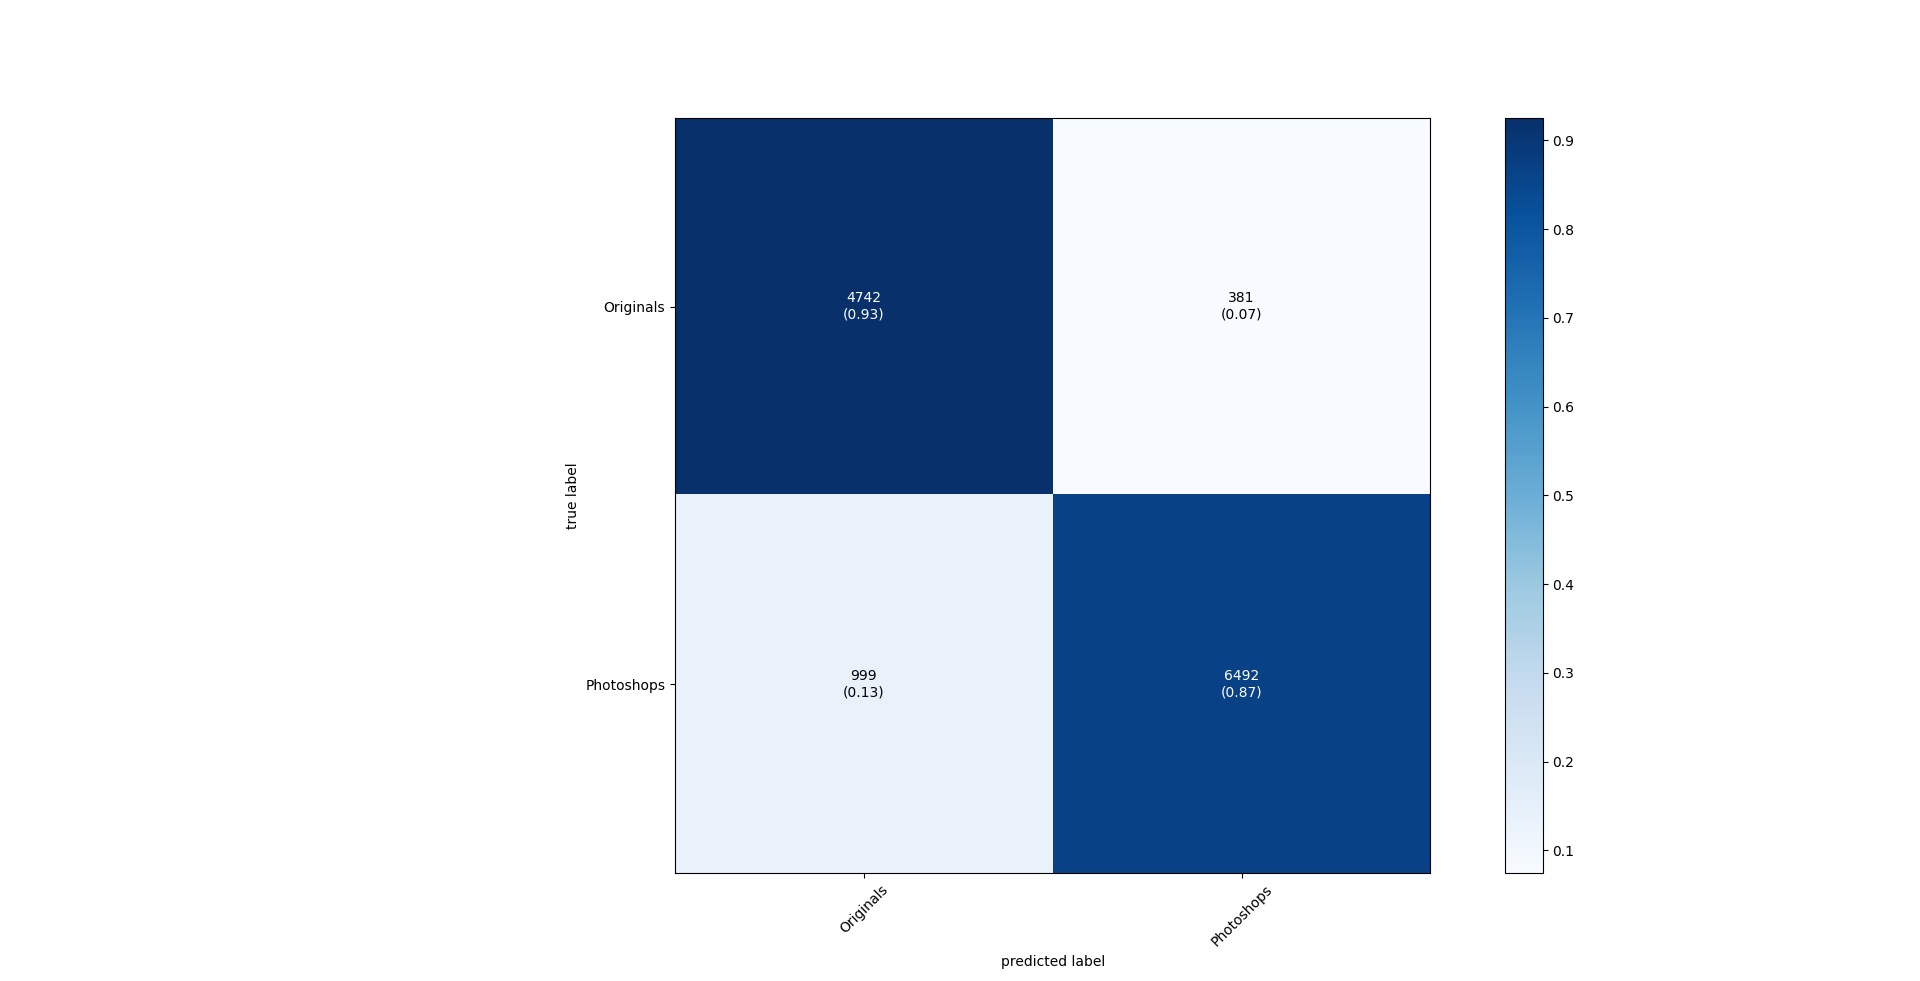
\includegraphics[width=10cm]{VGG_CASIA_CM.png}
	\centering
	\caption{Tablica błędów dla VGG16, trenowanego na zbiorze danych CASIA}
	\label{fig:vgg_cm_casia}
\end{figure}
\begin{figure}[h!]
	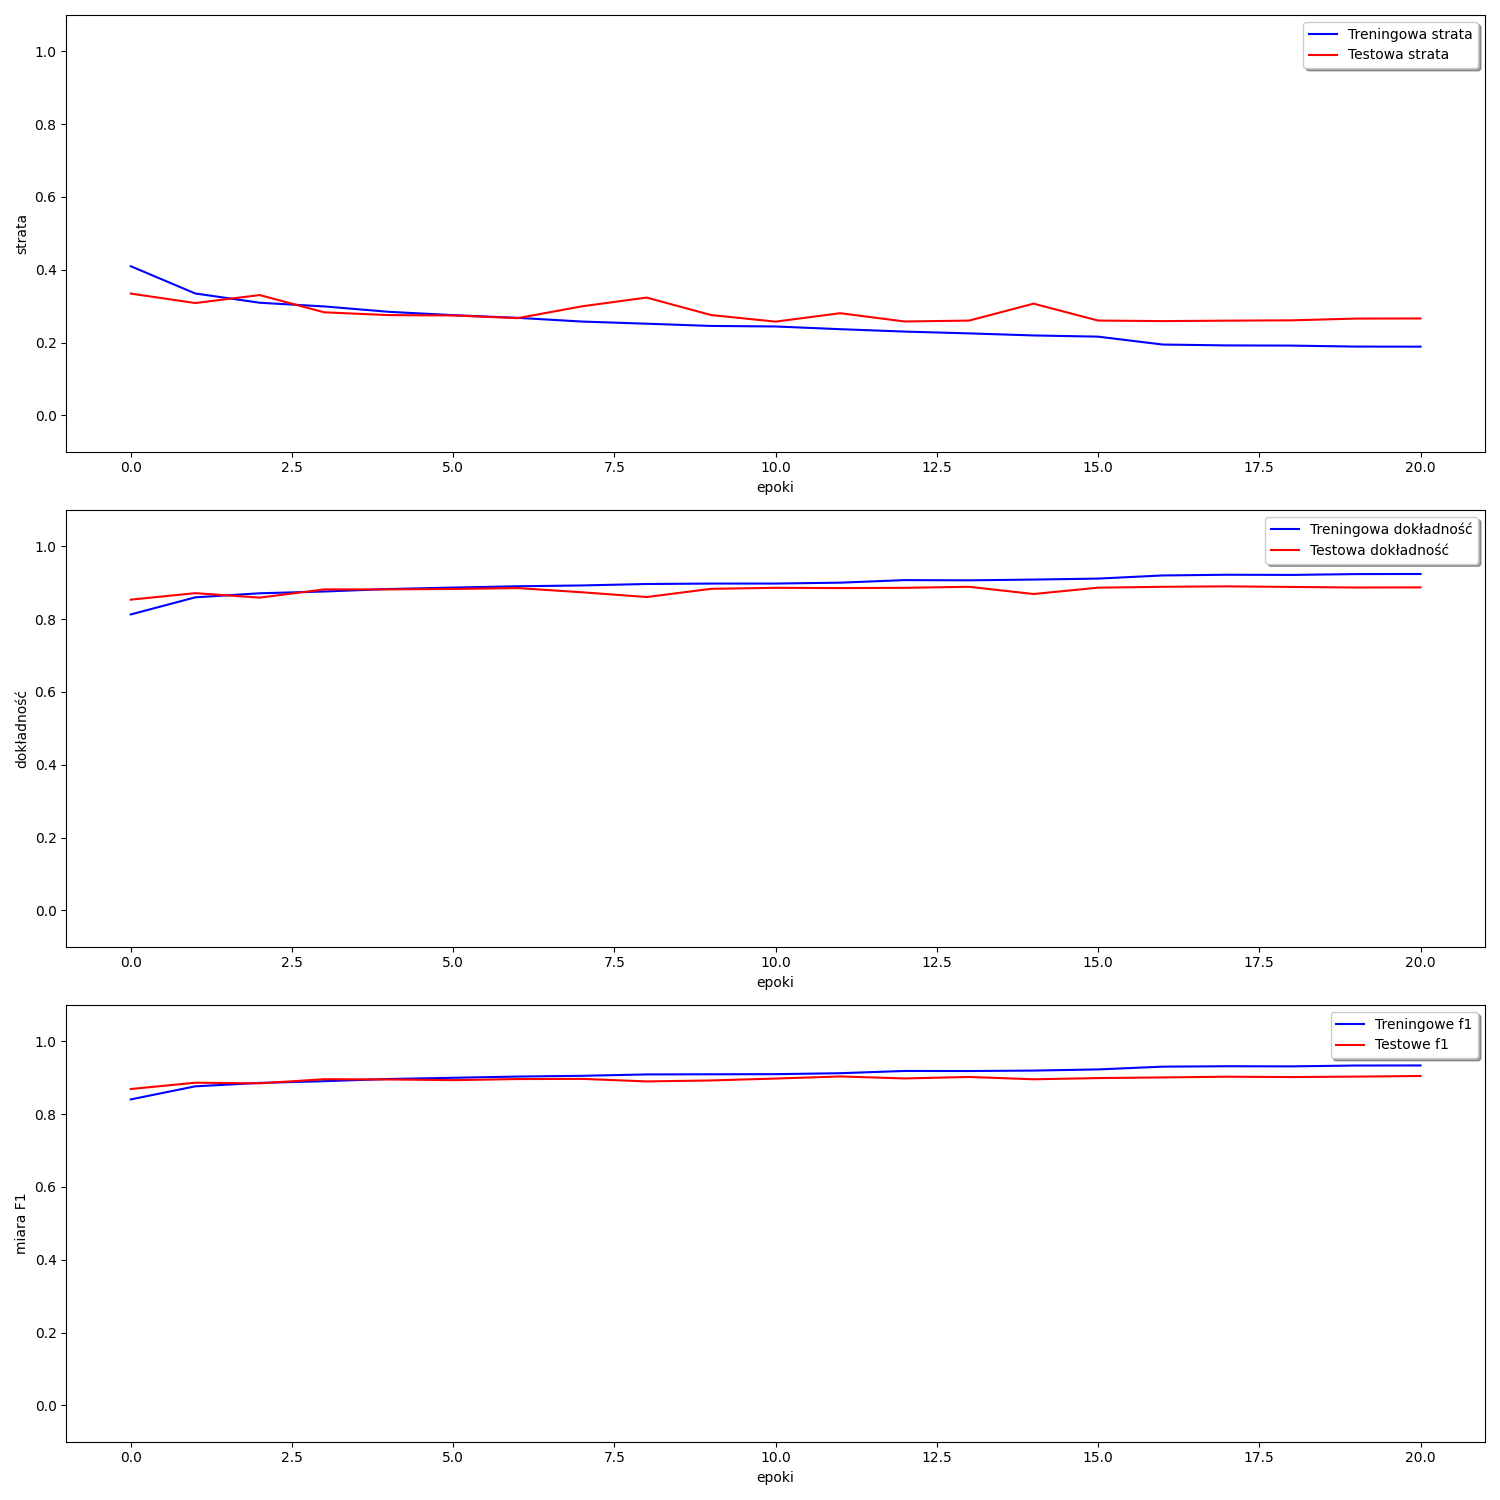
\includegraphics[width=13cm]{vgg_casia.png}
	\centering
	\caption{Przebieg uczenia dla VGG16, trenowanego na zbiorze danych CASIA}
	\label{fig:vgg_learn_casia}
\end{figure}

\textbf{Zbiór danych PS-Battles} \\

Same wyniki są przestawione w tabeli \ref{tab:result_p_vgg}. Podano tam wartość danej statystyki(liczoną jako średnią z pięciu przebiegów) oraz dodatkowo odchylenie standardowe.
\begin{table}[h!]
	\centering
	\begin{tabular}{|l|l|}
		\hline
		\textbf{Kernel}     & VGG          \\ \hline
		\textbf{Dokładność} & 0.689 (0.01) \\ \hline
		\textbf{Precyzja}   & 0.696 (0.01) \\ \hline
		\textbf{Czułość}    & 0.674 (0.02) \\ \hline
		\textbf{Miara \textit{F}}    & 0.684 (0.00) \\ \hline
	\end{tabular}
	\caption{Wartości szeregu miar dla modelu opartego o VGG16, trenowanego na zbiorze danych PS-Battles}
	\label{tab:result_p_vgg}
\end{table}

Tablica błędów została przedstawiona na rysunku \ref{fig:vgg_cm_ps}, a przebieg funkcji uczących na rysunku \ref{fig:vgg_learn_photo}.

\begin{figure}[h!]
	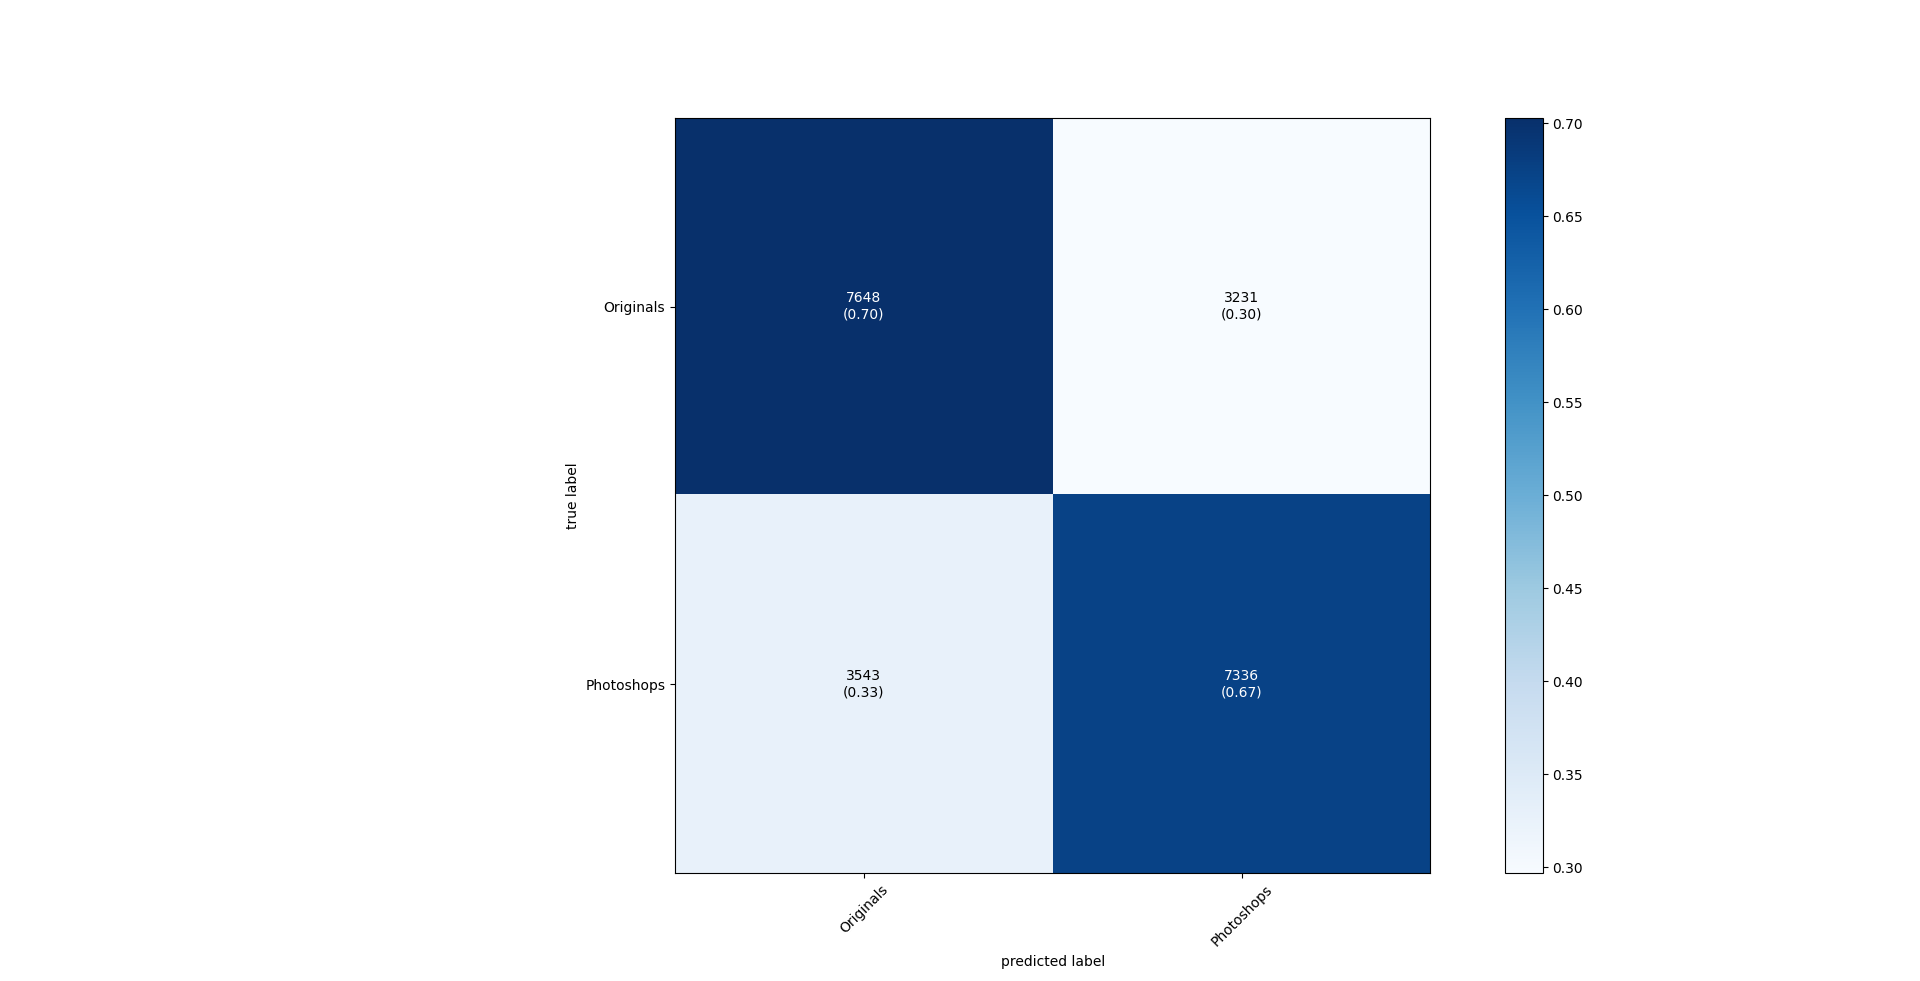
\includegraphics[width=10cm]{VGG_PHOTO_CM.png}
	\centering
	\caption{Tablica błędów dla VGG16, trenowanego na zbiorze danych PS-Battles}
	\label{fig:vgg_cm_ps}
\end{figure}
\begin{figure}[h!]
	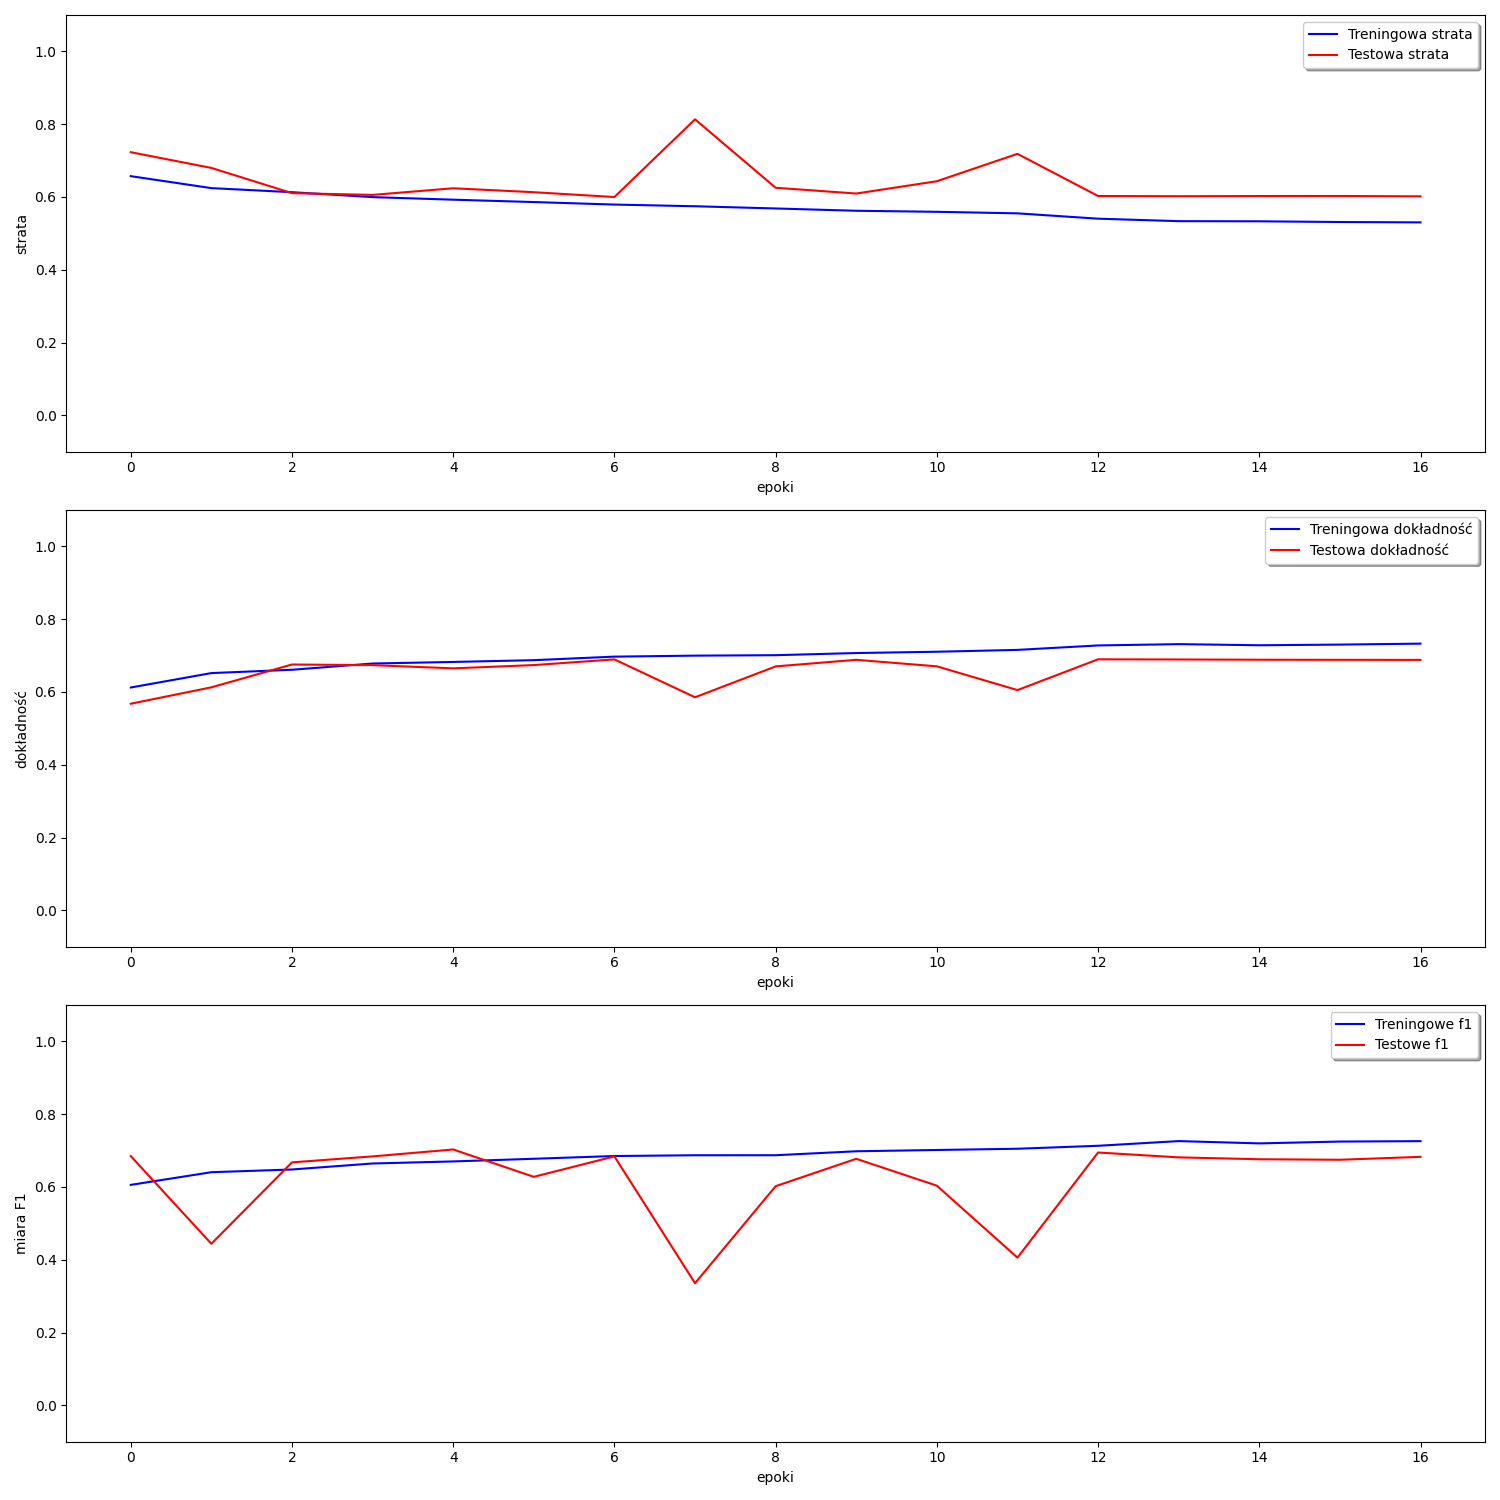
\includegraphics[width=13cm]{vgg_photo.png}
	\centering
	\caption{Przebieg uczenia dla VGG16, trenowanego na zbiorze danych PS-Battles}
	\label{fig:vgg_learn_photo}
\end{figure}

\section{Implementacja autorskiej metody wykorzystania uczenia głębokiego w zadaniu klasyfikacji}

Ostatnim klasyfikatorem na jaki się zdecydowałem jest autorska splotowa sieć neuronowa. Schemat używanego przez ze mnie modelu dostępny jest na rysunku \ref{fig:cnn}

\begin{figure}[h!]
	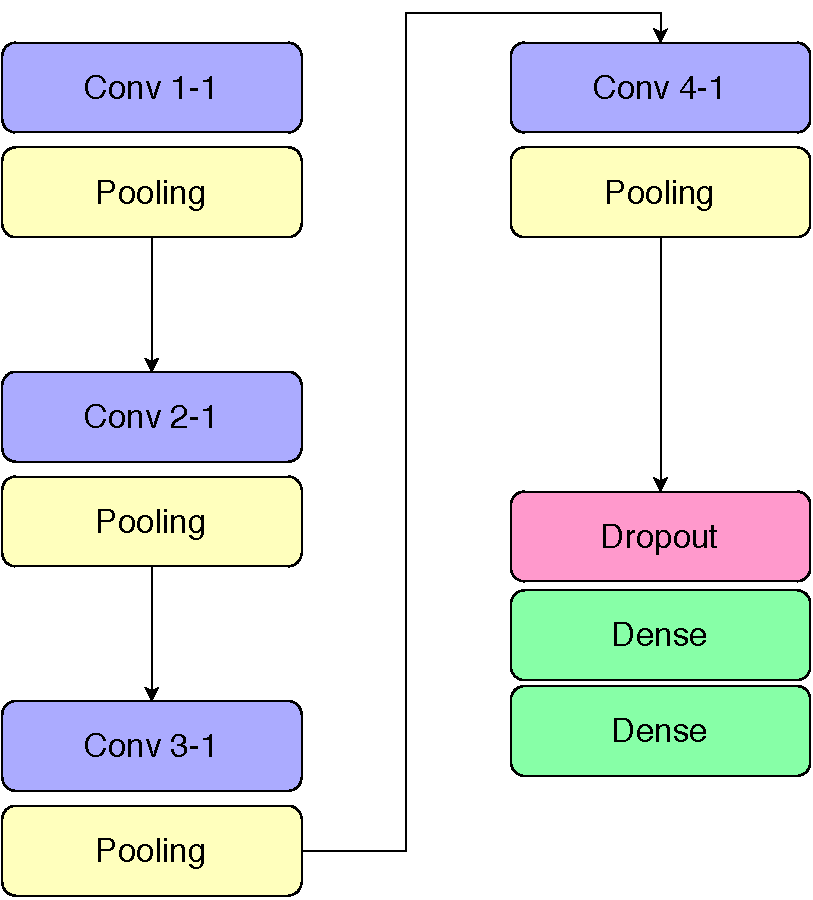
\includegraphics[width=8cm]{cnn.pdf}
	\centering
	\caption{Schemat autorskiego modelu CNN}
	\label{fig:cnn}
\end{figure}

\subsection{Przygotowanie danych}

Sam sposób przygotowania i obróbki danych jest bliźniaczy co na rozwiązaniu wykorzystującym sieć VGG Net - nie jest wykonywana żadna ekstrakcja cech, a jedyne co jest robione to zmiana zdjęcia z oryginalnego na jego wersję przetworzoną przez algorytm ELA, którego kod dostępny jest na listingu \ref{lst:ela}, oraz w formacie graficznej reprezentacji na rysunku \ref{fig:ela}. Wielkość zdjęcia została ustalona na $128 \times 128$.

\subsection{Definicja i uczenie modelu}

Uczony model jest zgodny z jego graficzną reprezentacją na rysunku \ref{fig:cnn}. Oczywiście podobnie jak w przypadku VGG Netu - mamy tu do czynienia z szeregiem parametrów sterujących, przedstawionych na listingu \ref{lst:cnn_param}:

\begin{lstlisting}[caption={Parametry pracy autorskiego modelu CNN}, label={lst:cnn_param}]
epochs = 50
batch_size = 100
activation = 'relu'
loss_type = 'binary_crossentropy'
optimizer = RMSprop(lr=1e-4)
dropout = 0.25
\end{lstlisting}

Idea trzech odpowiedzi zwrotnych sterujących procesem uczenia jest również tu obecna i bliźniacza jak do rozwiązania VGG Netowego, dostępnego na listningu \ref{lst:call}. Wszystkie parametry każdego z trzech procesów są ustawione dokładnie tak samo jak tam. 

\subsection{Interpretacja uzyskanych wyników}

Poniżej przedstawiam wyniki uzyskane dla poszczególnych zbiorów danych jakie zostały użyte podczas pisania pracy.\\

\textbf{Zbiór danych CASIA} \\

Same wyniki są przestawione w tabeli \ref{tab:result_cnn}. Podano tam wartość danej statystyki(liczoną jako średnią z pięciu przebiegów) oraz dodatkowo odchylenie standardowe. Tablica błędów i przebieg funkcji uczących zostały przedstawione na rysunku \ref{fig:cnn_cm_casia}. \\
\begin{table}[h!]
	\centering
	\begin{tabular}{|l|l|l|l|l|}
		\hline
		\textbf{Kernel} & \textbf{Dokładność} & \textbf{Precyzja} & \textbf{Czułość} & \textbf{Miara \textit{F}} \\ \hline
		CNN             & 0.909 (0.01)        & 0.962 (0.01)      & 0.882 (0.01)     & 0.920 (0.01)     \\ \hline
	\end{tabular}
	\caption{Wartości szeregu miar dla modelu opartego o autorskie rozwiązanie CNN, trenowanego na zbiorze danych CASIA}
	\label{tab:result_cnn}
\end{table}

\begin{figure}[h!]
	\centering
	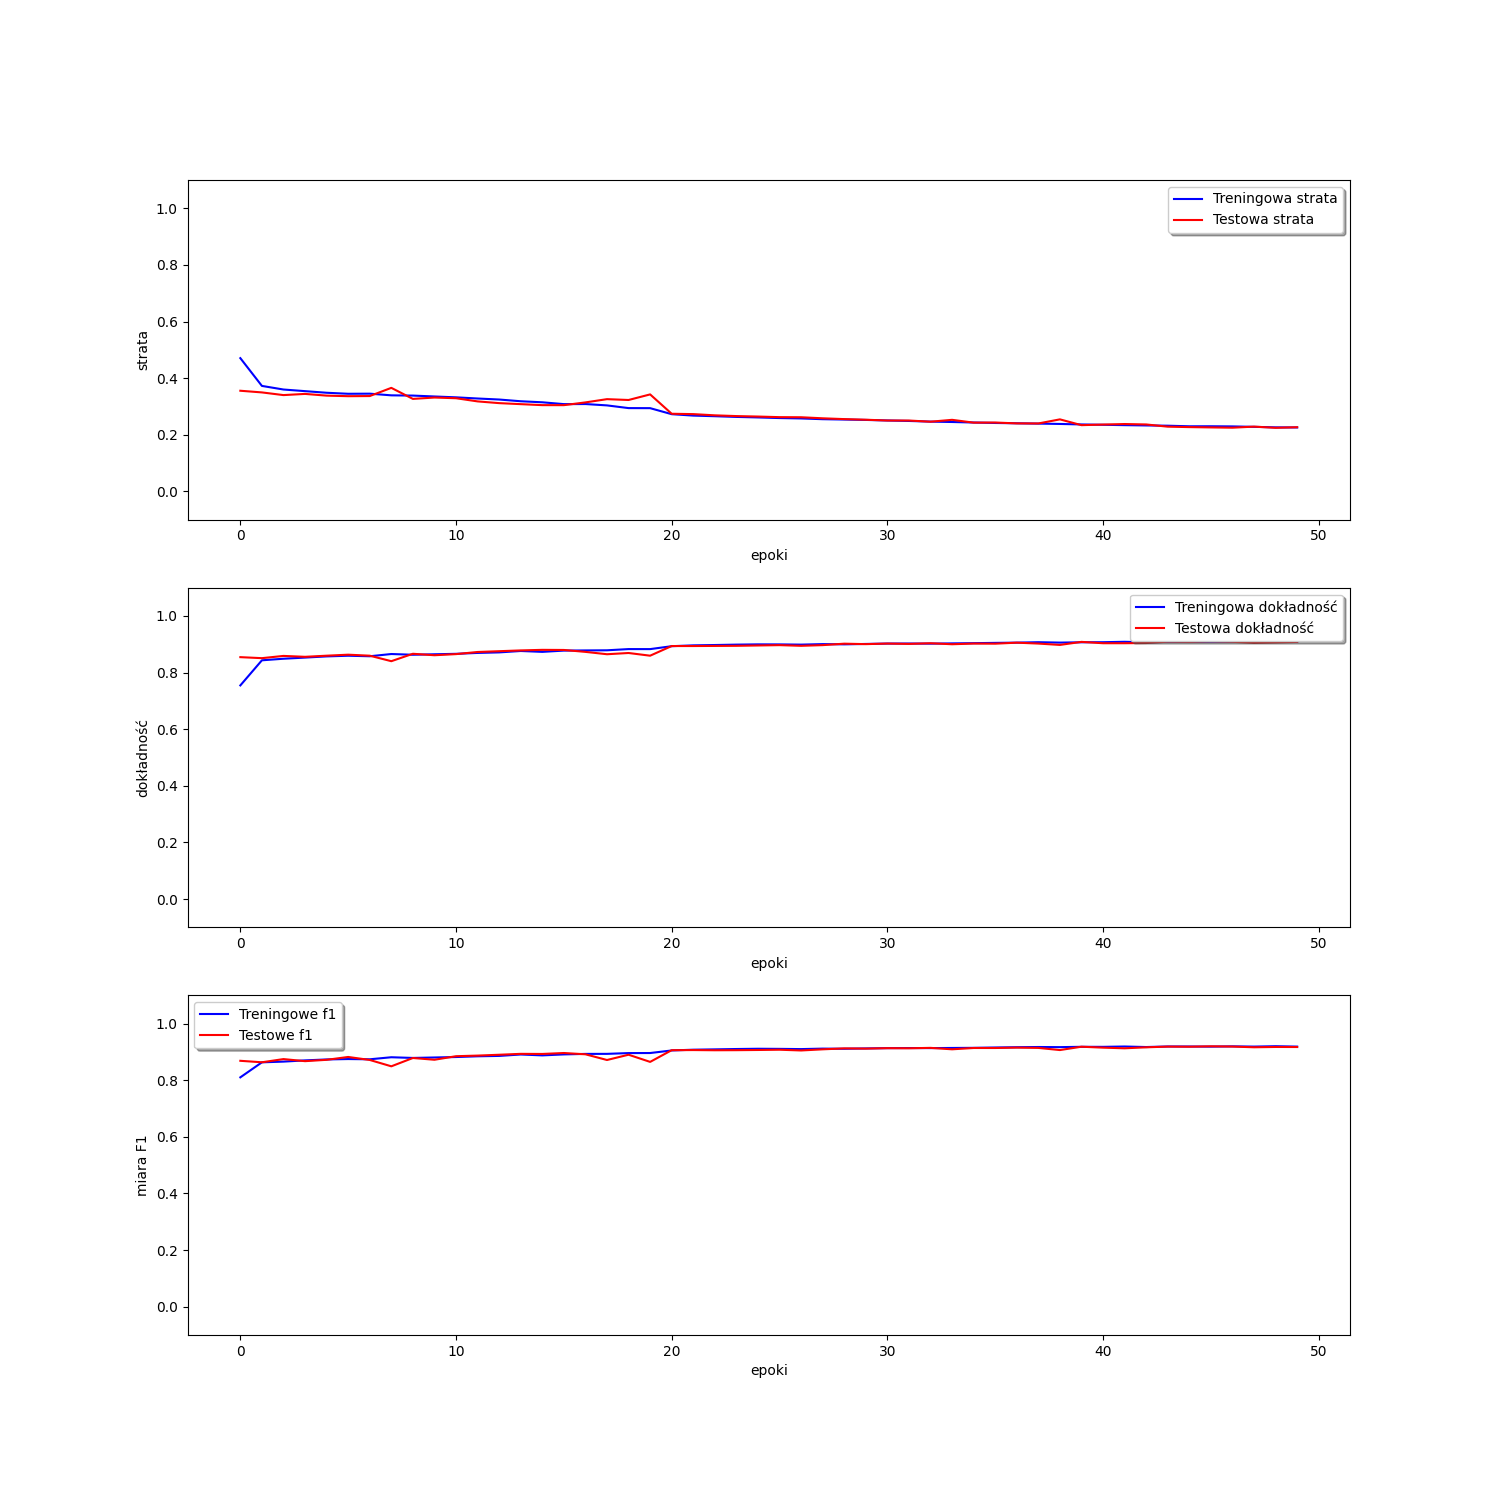
\includegraphics[width=15cm]{cnn_casia.png}
	\caption{Tablica błędów(lewo) i Przebiegi uczenia(prawo) dla autorskiego rozwiązania CNN}
	\label{fig:cnn_cm_casia}
\end{figure}

\textbf{Zbiór danych PS-Battles} \\

Same wyniki są przestawione w tabeli \ref{tab:result_p_cnn}. Podano tam wartość danej statystyki(liczoną jako średnią z pięciu przebiegów) oraz dodatkowo odchylenie standardowe. Tablica błędów i przebieg funkcji uczących zostały przedstawione na rysunku \ref{fig:cnn_cm_photo}.
\begin{table}[h!]
	\centering
	\begin{tabular}{|l|l|l|l|l|}
		\hline
		\textbf{Kernel} & \textbf{Dokładność} & \textbf{Precyzja} & \textbf{Czułość} & \textbf{Miara \textit{F}} \\ \hline
		CNN             & 0.706 (0.01)        & 0.711 (0.01)      & 0.697 (0.01)     & 0.704 (0.01)     \\ \hline
	\end{tabular}
	\caption{Wartości szeregu miar dla modelu opartego o autorskie rozwiązanie CNN, trenowanego na zbiorze danych PS-Battles}
	\label{tab:result_p_cnn}
\end{table}

\begin{figure}[h!]
	\centering
	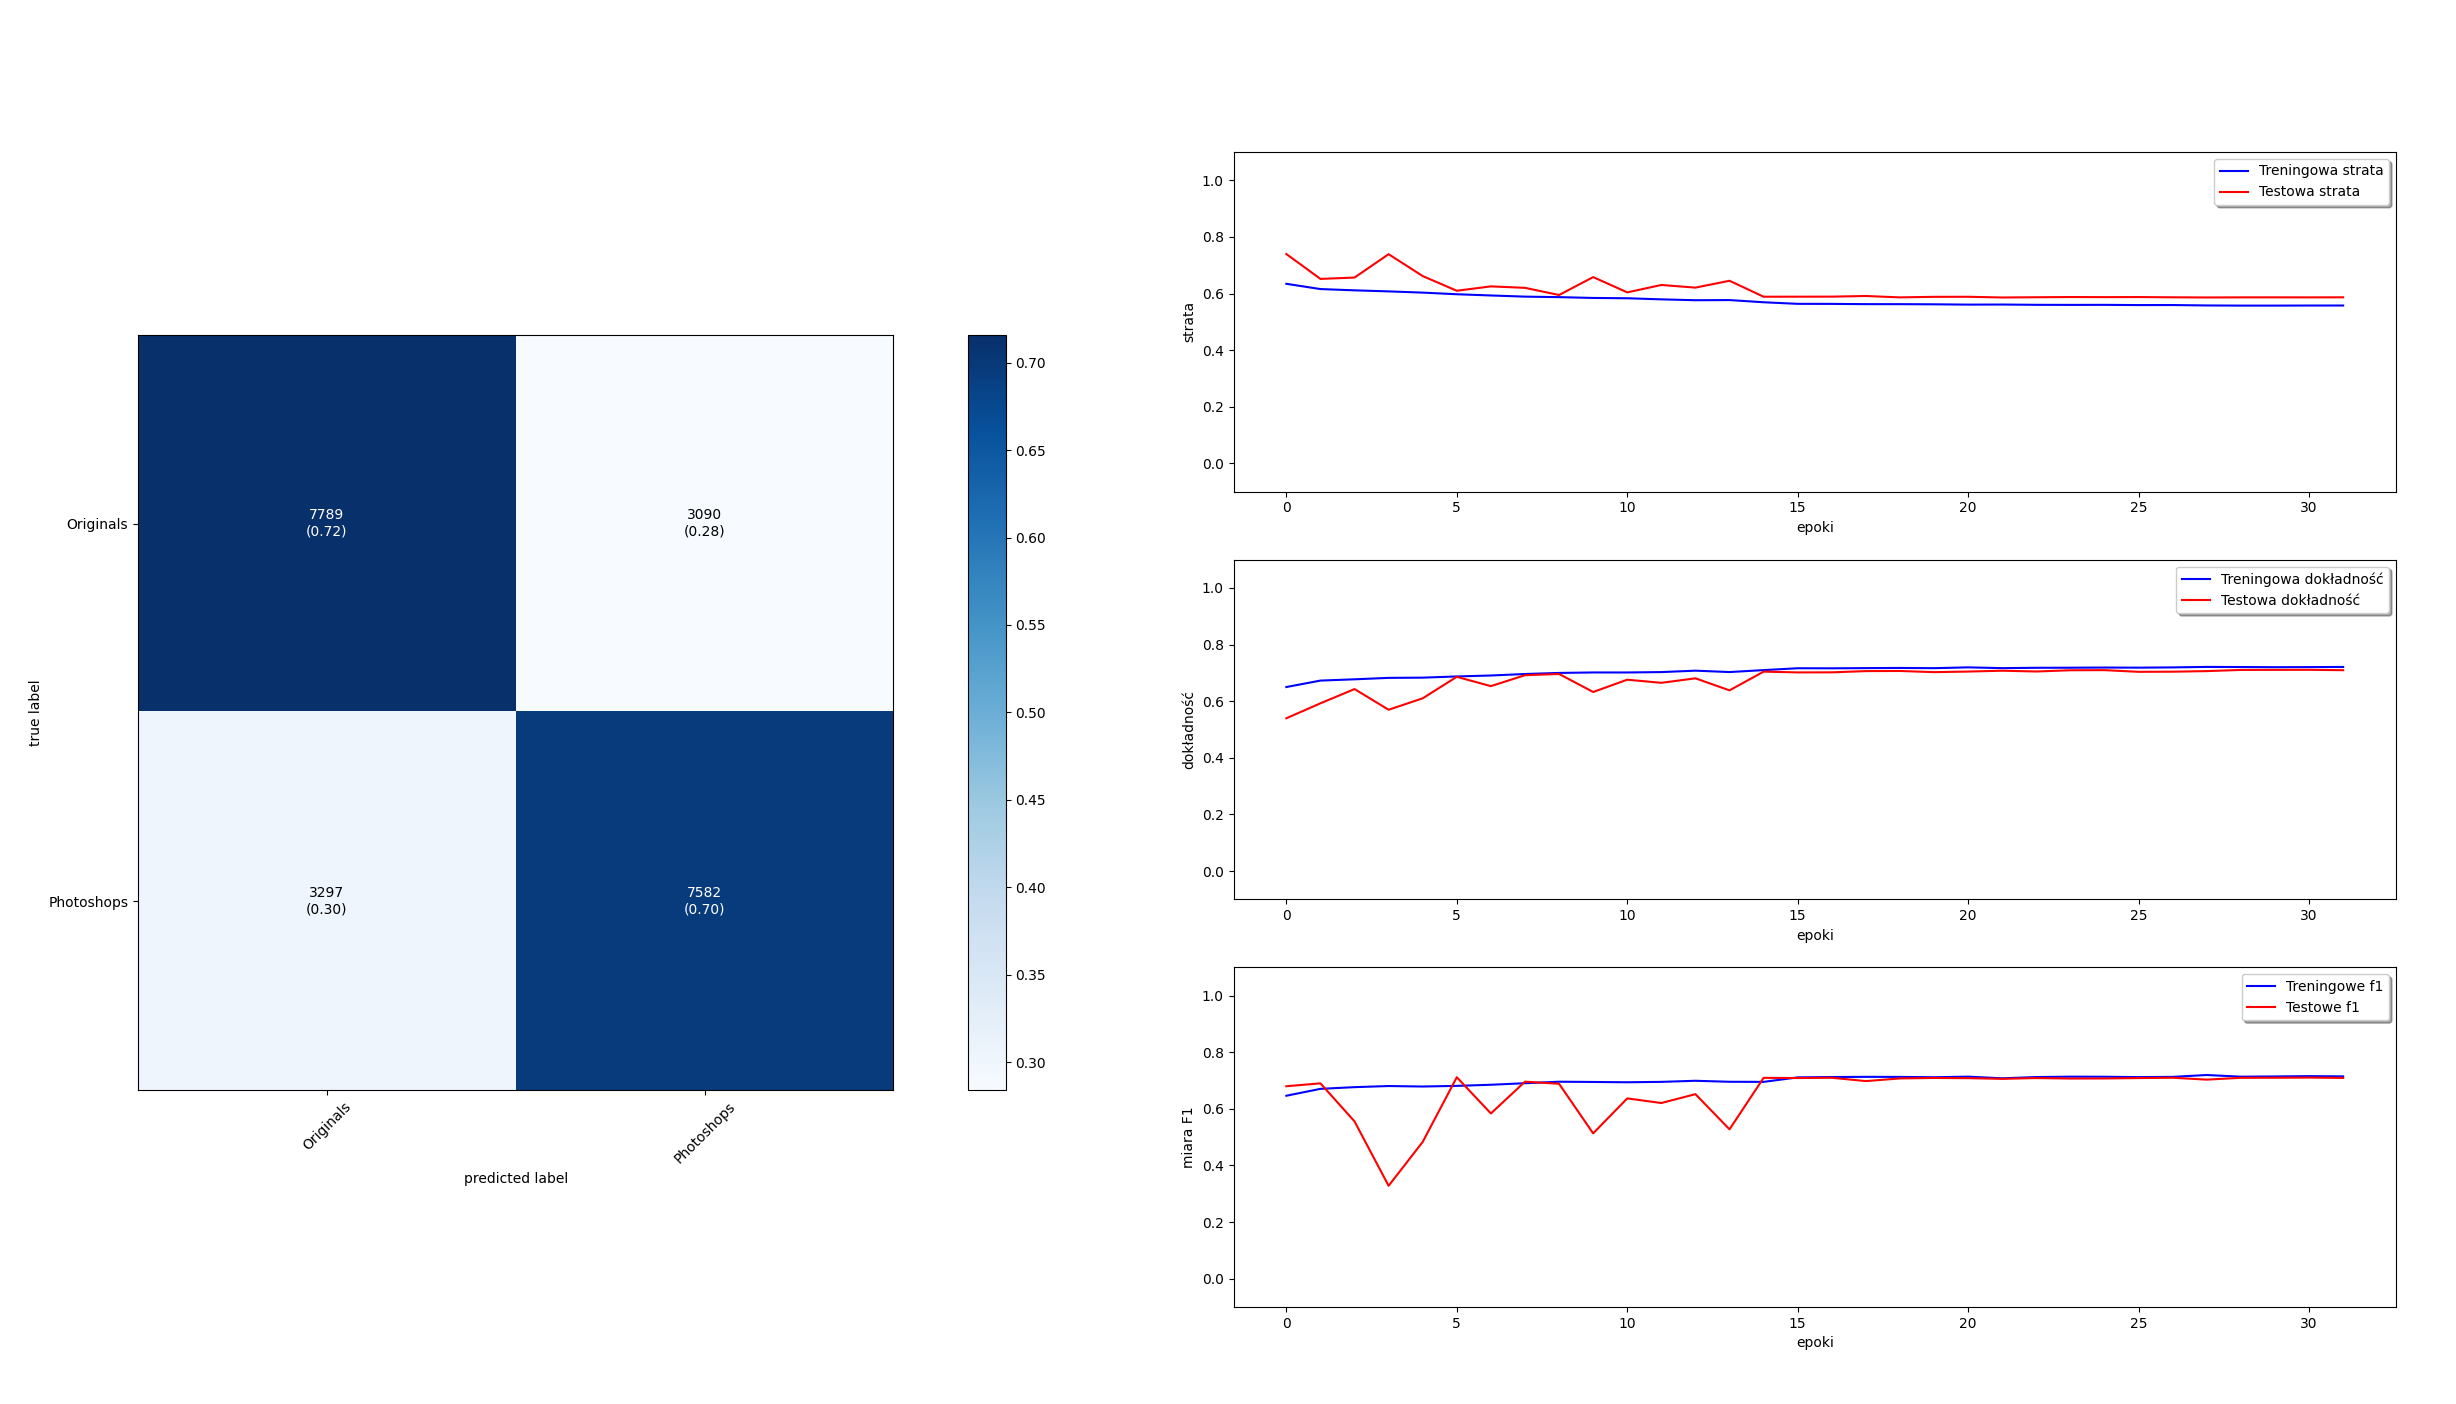
\includegraphics[width=15cm]{cnn_photo.png}
	\caption{Tablica błędów(lewo) i Przebiegi uczenia(prawo) dla autorskiego rozwiązania CNN}
	\label{fig:cnn_cm_photo}
\end{figure}

\section {Przedstawienie i omówienie uzyskanych wyników}

W tabeli \ref{tab:all_result} przedstawiam rezultaty dla wszystkich mierzonych statystyk, wszystkich modeli i obu zbiorów danych:

\begin{table}[h!]
	\centering
	\begin{tabular}{l|l|l|l|l|l|}
		\cline{2-6}
		& \textbf{Kernel} & \textbf{Dokładność} & \textbf{Precyzja} & \textbf{Czułość} & \textbf{Miara \textit{F}} \\ \hline
		\multicolumn{1}{|c|}{\multirow{3}{*}{\textbf{CASIA}}}       & \textit{SVM} & 0.725 (0.00) & 0.669 (0.00) & 0.638 (0.01) & 0.653 (0.00) \\ \cline{2-6} 
		\multicolumn{1}{|c|}{} & \textit{VGG}    & 0.891 (0.01)        & 0.945 (0.01)      & 0.867 (0.01)     & 0.904 (0.01)     \\ \cline{2-6} 
		\multicolumn{1}{|c|}{} & \textit{CNN}    & 0.909 (0.01)        & 0.962 (0.01)      & 0.882 (0.01)     & 0.920 (0.01)     \\ \hline
		\multicolumn{1}{|l|}{\multirow{3}{*}{\textbf{PS-Battles}}} & \textit{SVM} & 0.580 (0.01) & 0.590 (0.01) & 0.527 (0.01) & 0.557 (0.01) \\ \cline{2-6} 
		\multicolumn{1}{|l|}{} & \textit{VGG}    & 0.689 (0.01)        & 0.696 (0.02)      & 0.674 (0.02)     & 0.684 (0.00)     \\ \cline{2-6} 
		\multicolumn{1}{|l|}{} & \textit{CNN}    & 0.706 (0.01)        & 0.711 (0.01)      & 0.697 (0.01)     & 0.704 (0.01)     \\ \hline
	\end{tabular}
	\caption{Zbiorcze wyniki miar dla wszystkich policzonych modeli i zbiorów danych}
	\label{tab:all_result}
\end{table}

Wyniki parowych testów statystycznych dla wszystkich modeli i miar dostępne są w tabelach \ref{tab:t_results} i \ref{tab:t_results_p}. Pierwsza z nich przedstawia wyniki dla zbioru danych CASIA, a druga tabela pokazuje rezultaty dla zbioru danych PS-Battles.

\begin{table}[h!]
	\centering
	\begin{tabular}{l|l|l|l|l|l|l|l|l|l|l|l|l|}
		\cline{2-13}
		&
		\multicolumn{3}{c|}{\textbf{Dokładność}} &
		\multicolumn{3}{c|}{\textbf{Precyzja}} &
		\multicolumn{3}{c|}{\textbf{Czułość}} &
		\multicolumn{3}{c|}{\textbf{Miara \textit{F}}} \\ \cline{2-13} 
		&
		\textbf{S} &
		\textbf{V} &
		\textbf{C} &
		\textbf{S} &
		\textbf{V} &
		\textbf{C} &
		\textbf{S} &
		\textbf{V} &
		\textbf{C} &
		\textbf{S} &
		\textbf{V} &
		\textbf{C} \\ \hline
		\multicolumn{1}{|l|}{\textbf{SVM}} & 0 & 0 & 0 & 0 & 0 & 0 & 0 & 0 & 0 & 0 & 0 & 0 \\ \hline
		\multicolumn{1}{|l|}{\textbf{VGG}} & 1 & 0 & 0 & 1 & 0 & 0 & 1 & 0 & 0 & 1 & 0 & 0 \\ \hline
		\multicolumn{1}{|l|}{\textbf{CNN}} & 1 & 1 & 0 & 1 & 1 & 0 & 1 & 0 & 0 & 1 & 1 & 0 \\ \hline
	\end{tabular}
	\caption{Wyniki parowego testu statystycznego dla zbioru danych Casia}
	\label{tab:t_results}
\end{table}

\begin{table}[h!]
	\centering
	\begin{tabular}{l|l|l|l|l|l|l|l|l|l|l|l|l|}
		\cline{2-13}
		&
		\multicolumn{3}{c|}{\textbf{Dokładność}} &
		\multicolumn{3}{c|}{\textbf{Precyzja}} &
		\multicolumn{3}{c|}{\textbf{Czułość}} &
		\multicolumn{3}{c|}{\textbf{Miara \textit{F}}} \\ \cline{2-13} 
		&
		\textbf{S} &
		\textbf{V} &
		\textbf{C} &
		\textbf{S} &
		\textbf{V} &
		\textbf{C} &
		\textbf{S} &
		\textbf{V} &
		\textbf{C} &
		\textbf{S} &
		\textbf{V} &
		\textbf{C} \\ \hline
		\multicolumn{1}{|l|}{\textbf{SVM}} & 0 & 0 & 0 & 0 & 0 & 0 & 0 & 0 & 0 & 0 & 0 & 0 \\ \hline
		\multicolumn{1}{|l|}{\textbf{VGG}} & 1 & 0 & 0 & 1 & 0 & 0 & 1 & 0 & 0 & 1 & 0 & 0 \\ \hline
		\multicolumn{1}{|l|}{\textbf{CNN}} & 1 & 1 & 0 & 1 & 0 & 0 & 1 & 0 & 0 & 1 & 1 & 0 \\ \hline
	\end{tabular}
	\caption{Wyniki parowego testu statystycznego dla zbioru danych PS-Battles}
	\label{tab:t_results_p}
\end{table}

Jak widać najlepsze wyniki, które są statystycznie znaczące, osiągnęło moje autorskie rozwiązanie. Uzyskując kolejno $\sim91\%$ dokładność dla zbioru CASIA i $\sim71\%$ dokładności dla zbioru PS-Battles.
